
\documentclass[preprint,12pt,authoryear]{elsarticle}

\usepackage[T1]{fontenc}
\usepackage[utf8]{inputenc}
\usepackage[english]{babel}
\usepackage{lmodern}

\usepackage[top=2.5cm, bottom=2.5cm, left=3cm, right=2.5cm]{geometry}
\usepackage{setspace}
\onehalfspacing
\usepackage{parskip}            
\usepackage{microtype}         
\sloppy

\usepackage{amsmath}
\usepackage{amssymb}
\usepackage{graphicx}
\usepackage{float}
\usepackage{booktabs}
\usepackage{tabularx}
\usepackage{caption}
\captionsetup{font=small, labelfont=bf, skip=6pt}

\usepackage{siunitx}
\usepackage{enumitem}
\usepackage{lineno}             
\linenumbers
\usepackage[colorlinks=true,
linkcolor=blue,
citecolor=blue,
urlcolor=blue]{hyperref}
\newcommand{\doi}[1]{\textsc{doi}: \href{https://doi.org/#1}{#1}}

\journal{Remote Sensing Applications: Society and Environment}

\begin{document}
	
	\begin{frontmatter}
		
		\title{Spatio-Temporal Cluster Detection of Forest Fires in Southern Peru (2017--2025) Using the SaTScan Method and Spatial Autocorrelation}
		
		\author[1]{Jhon Cristhian Gonzales Quispe\corref{cor1}}
		\ead{j.gonzales@est.unap.edu.pe}
		\cortext[cor1]{Corresponding author}
		\address[1]{Universidad Nacional del Altiplano, Puno, Peru}
		
		\begin{abstract}
			Forest fires are a growing threat to Peru's Andean-Amazonian
			ecosystems. This study detects and characterizes spatio-temporal
			clusters of forest fires in southern Peru (Madre de Dios, Puno, and
			Cusco) during 2017--2025, integrating 74{,}861 satellite-derived
			thermal anomalies (NASA FIRMS VIIRS/MODIS) and 2{,}727{,}647
			deforestation alerts (GeoBosques-MINAM) at the district and monthly
			level. A discrete Poisson spatio-temporal scan model (SaTScan) was
			applied, complemented by global (Moran's Index) and local
			(univariate and bivariate LISA) spatial autocorrelation analysis,
			together with sensitivity tests using 25\,\%, 30\,\%, and 50\,\%
			spatial windows. Results reveal extreme seasonality, with 89.51\,\%
			of events concentrated between July and October (peak in September:
			39.01\,\%), and two interannual maxima coinciding with severe
			droughts and El Ni\~no episodes (2020 and 2024). Nine statistically
			significant spatio-temporal clusters were identified
			($p < 0.00001$). The primary cluster was located at the
			Cusco--Puno Andean interface (96 districts, 2019--2022,
			$\text{LLR} = 35{,}231.2$, $\text{RR} = 780.02$), whereas Madre de
			Dios concentrated the highest absolute fire burden within Amazonian
			clusters (Cluster~4: 14{,}264 fires; Cluster~6: 15{,}863 fires). The
			bivariate Moran's Index ($I = 0.6019$, $p = 0.001$) confirmed a
			strong spatial dependence between prior deforestation and fire
			occurrence in neighboring districts, and sensitivity analyses
			confirmed the full stability of the primary cluster. These findings
			provide key empirical evidence for prioritizing intervention zones
			and early-warning systems by Peru's forestry and environmental
			authorities (SERFOR and MINAM).
		\end{abstract}
		
		\begin{keyword}
			Spatial statistics \sep SaTScan \sep Forest fires \sep Deforestation \sep Spatial autocorrelation \sep LISA \sep Southern Peru
		\end{keyword}
		
	\end{frontmatter}
	
	\section{Introduction}
	
	Forest fires constitute one of the main environmental threats to
	the Amazonian and Andean ecosystems of South America, with direct
	consequences for biodiversity, air quality, the health of local
	populations, and greenhouse gas emissions~\citep{Aragao2018,Nepstad1999,Cochrane2003}.
	In Peru, the frequency and intensity of these events have
	intensified over the last decade, driven by the expansion of the
	agricultural frontier, traditional burning practices for land-use
	change, and prolonged drought periods associated with climatic
	phenomena such as El Ni\~no~\citep{SERFOR2023,Mostiga2026,Marengo2011}.
	The southern regions of the country ---Madre de Dios, Puno, and
	Cusco--- concentrate a significant share of these events owing to
	their vast Amazonian forest cover and the persistence of
	agropastoral burning practices in forest-human interface
	zones~\citep{MINAM2024,Barboza2024,Zubieta2021}. At the continental
	level, the 2019 fire crisis revealed severe positive anomalies in
	the Peruvian Amazon and the central Andes, with burned area
	exceeding the historical average by 70\,\%~\citep{Lizundia2020}.
	Recent studies in the Brazilian Amazon confirm that proximity to
	roads and pasture expansion are the main anthropogenic drivers of
	spatio-temporal fire clusters~\citep{Valente2023,Raiol2026,BolanoDiaz2022}.
	
	Spatial statistics has proven to be an effective tool for
	characterizing the geographic distribution of environmental
	phenomena and detecting non-random clustering patterns in space and
	time. Among the available methods, SaTScan ---based on spatial and
	spatio-temporal scanning using discrete probability models---
	allows the identification of statistically significant clusters of
	events as well as their temporal evolution, which is particularly
	useful for anticipating the expansion of fire foci and prioritizing
	intervention areas~\citep{Kulldorff1997,Kulldorff2001,VegaOrozco2012,Urfali2025,Zerbe2022}.
	This method has been successfully applied to forest fires in Europe
	and the Brazilian Amazon~\citep{VegaOrozco2012,Valente2023}, although
	its use in the Peruvian context ---outside the domain of public
	health--- remains scarce. In addition, Moran's Index and Local
	Indicators of Spatial Association (LISA) allow the identification of
	hot spots and significant spatial anomalies in environmental
	phenomena such as forest fires, including in bivariate form to
	relate two contiguous geospatial
	variables~\citep{Anselin1995,Ma2022,Atalay2025}.
	
	In this context, the present study aims to detect and characterize
	the spatio-temporal clusters of forest fires that occurred in
	southern Peru during the period 2017--2025, by applying the SaTScan
	method and spatial autocorrelation indicators (Moran and LISA),
	contrasting their location with drought periods and forest-cover-loss
	alerts, in order to provide useful evidence for prioritizing fire
	prevention and response strategies in the region.
	
	\section{Study Area and Data Sources}
	
	\subsection{Study Area}
	
	The study area covers the southern sector of Peru, comprising the
	administrative regions of Madre de Dios, Puno, and Cusco
	(Figure~\ref{fig:mapa_densidad}). This macro-region transitions from
	the hyperdiverse Amazonian lowlands (Madre de Dios) to the Andean
	mountain range and the Lake Titicaca basin (Cusco and Puno),
	encompassing a political-administrative division of \textbf{237
		districts}.
	
	\begin{figure}[htbp]
		\centering
		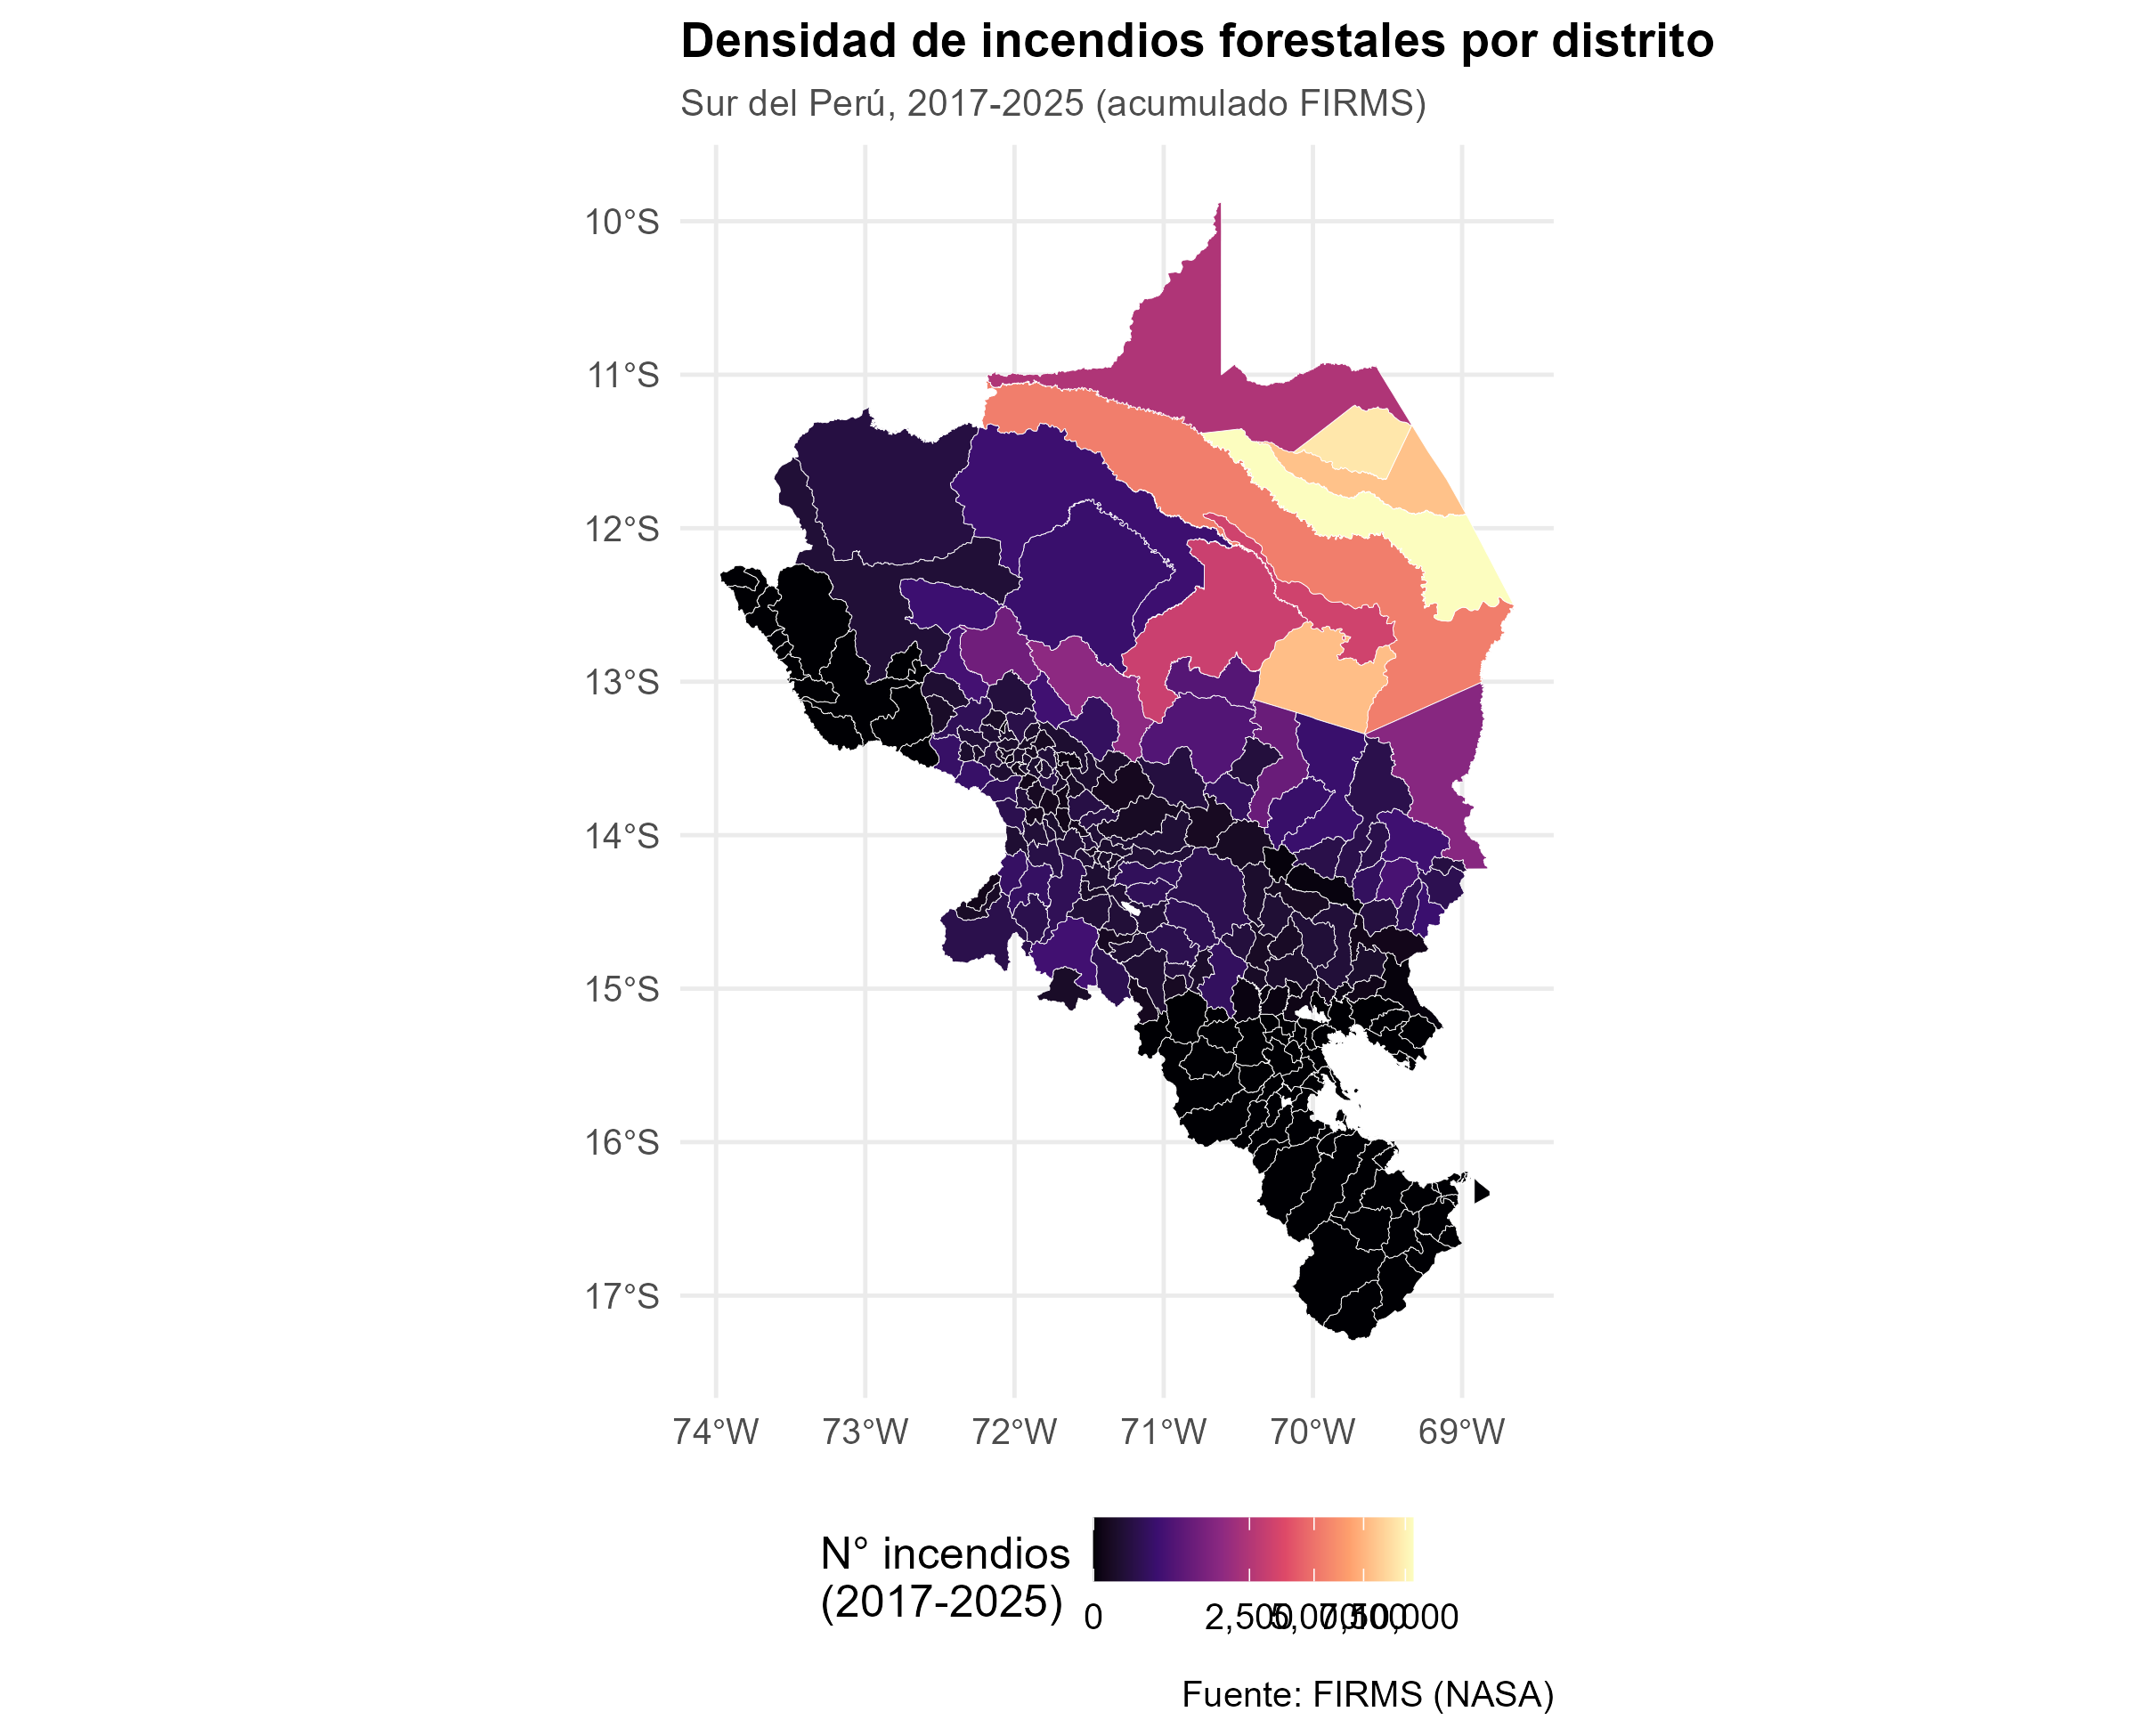
\includegraphics[width=0.85\textwidth]{mapa_densidad_incendios.png}
		\caption{Absolute density map of forest fires by district
			in southern Peru (2017--2025).}
		\label{fig:mapa_densidad}
	\end{figure}
	
	\subsection{Fire Hotspots (FIRMS)}
	
	Georeferenced point records from the VIIRS (SNPP/NOAA-20) and MODIS
	sensors were obtained from NASA's FIRMS system for the period from
	January 1, 2017 to December 31, 2025~\citep{Giglio2016,Giglio2018,Schroeder2014}.
	Each hotspot record contains geographic coordinates, acquisition
	date (\textit{acq\_date}), brightness, and confidence level. After
	spatial aggregation and filtering within the district boundaries of
	the study area to isolate genuine forest-burning
	events~\citep{Deng2025,Su2023}, a total of \textbf{74{,}861 fire
		hotspots} were consolidated.
	
	\subsection{Deforestation Alerts (GeoBosques)}
	
	To represent the population at risk and land-use-change pressure,
	spatio-temporal data from MINAM's GeoBosques platform were
	processed. A total of \textbf{2{,}727{,}647 point deforestation
		alerts} occurring between 2017 and 2025 were consolidated. The
	distribution by department shows that Madre de Dios concentrates
	71.77\,\% of the total (1{,}957{,}718 alerts), followed by Cusco
	(18.31\,\%, 499{,}521 alerts) and Puno (9.91\,\%, 270{,}408
	alerts)~\citep{AlarconAguirre2022}.
	
	\section{Spatial-Statistical Methodology}
	
	\subsection{SaTScan Discrete Poisson Model}
	
	Spatio-temporal cluster detection was carried out using SaTScan
	v10.3.3 with \textbf{Kulldorff's discrete Poisson spatio-temporal
		model}~\citep{Kulldorff1997,Kulldorff2001,Aboushady2025}. This model
	has been validated for detecting spatio-temporal clusters of forest
	fires from satellite hotspot data, allowing structural (recurrent)
	fire regimes to be distinguished from extemporaneous
	episodes~\citep{VegaOrozco2012,LevinRector2024}. The number of fires
	$c_{it}$ in district $i$ and month $t$ is assumed to be Poisson
	distributed with expected parameter:
	\[
	\mu_{it} = p_{it} \cdot \frac{C}{P},
	\]
	where $p_{it}$ is the number of deforestation alerts (baseline
	risk), $C$ is the total number of fires across the whole study, and
	$P$ is the total accumulated deforestation.
	
	The spatio-temporal cylindrical scanning window $Z$ varies
	continuously in space (centroid and radius of the base circle) and
	in time (range of months). For each cylinder $Z$, the likelihood
	function under the alternative hypothesis of increased risk is:
	\begin{equation}
		L(Z) = \left(\frac{c_Z}{\mu_Z}\right)^{c_Z}
		\left(\frac{C - c_Z}{C - \mu_Z}\right)^{C - c_Z}
		\mathbf{1}(c_Z > \mu_Z),
		\label{eq:verosimilitud}
	\end{equation}
	where $c_Z$ is the number of observed fires within $Z$, $\mu_Z$ is
	the expected number, and $\mathbf{1}(\cdot)$ is the indicator
	function for excess risk. The Log-Likelihood Ratio statistic (LLR)
	is calculated as:
	\begin{equation}
		\text{LLR} = \ln\!\left(\frac{L(Z)}{L_0}\right)
		= c_Z \ln\!\left(\frac{c_Z}{\mu_Z}\right)
		+ (C-c_Z)\ln\!\left(\frac{C-c_Z}{C-\mu_Z}\right).
		\label{eq:llr}
	\end{equation}
	Statistical significance was determined using $999$ Monte Carlo
	simulations. The Relative Risk (RR) was estimated as:
	\begin{equation}
		\text{RR} = \frac{c_Z / \mu_Z}{(C - c_Z) / (C - \mu_Z)}.
		\label{eq:rr}
	\end{equation}
	
	\subsection{Global and Local Spatial Autocorrelation (Moran and LISA)}
	
	In addition, static spatial dependence was assessed using the
	univariate and bivariate \textbf{Global Moran's Index}
	($I$)~\citep{Anselin1995}:
	\begin{equation}
		I = \frac{N}{\displaystyle\sum_{i}\sum_{j} w_{ij}}
		\cdot
		\frac{\displaystyle\sum_{i=1}^{N}\sum_{j=1}^{N}
			w_{ij}(x_i - \bar{x})(y_j - \bar{y})}
		{\displaystyle\sum_{i=1}^{N}(x_i - \bar{x})^2},
		\label{eq:moran}
	\end{equation}
	where $w_{ij}$ represents the row-standardized spatial contiguity
	matrix (Queen criterion). To identify the exact location of hot
	spots (\textit{High-High}) and spatial anomalies, univariate and
	bivariate Local Indicators of Spatial Association (LISA) were
	calculated with 999 random permutations~\citep{Kumari2025,Mupfiga2022,MemisogluBaykal2025}.
	Spatial processing and modeling were carried out in the R
	statistical environment~\citep{RCoreTeam2024}, using specialized
	packages for spatial dependence analysis~\citep{Bivand2013,Bivand2018}.
	
	\subsection{Sensitivity Analysis}
	
	To evaluate the robustness of the detected clusters under different
	maximum spatial extent assumptions, the SaTScan analysis was
	repeated restricting the maximum spatial window to 25\,\% and
	30\,\% of the population at risk, complementing the baseline 50\,\%
	configuration.
	
	\section{Results}
	
	\subsection{Temporal Patterns and Seasonality}
	
	The temporal analysis (Figure~\ref{fig:serie_anual}) shows marked
	interannual variability, with two severe critical peaks in
	\textbf{2020} (12{,}811 fires) and \textbf{2024} (12{,}437 fires),
	coinciding with periods of extreme drought associated with El Ni\~no
	events. The aggregated monthly distribution
	(Figures~\ref{fig:estacionalidad} and~\ref{fig:heatmap}) reveals
	extreme concentration during the austral dry season: the months of
	July through October account for \textbf{89.51\,\%} of annual
	occurrence, peaking in \textbf{September (39.01\,\%)} and
	\textbf{August (25.22\,\%)}.
	
	\begin{figure}[htbp]
		\centering
		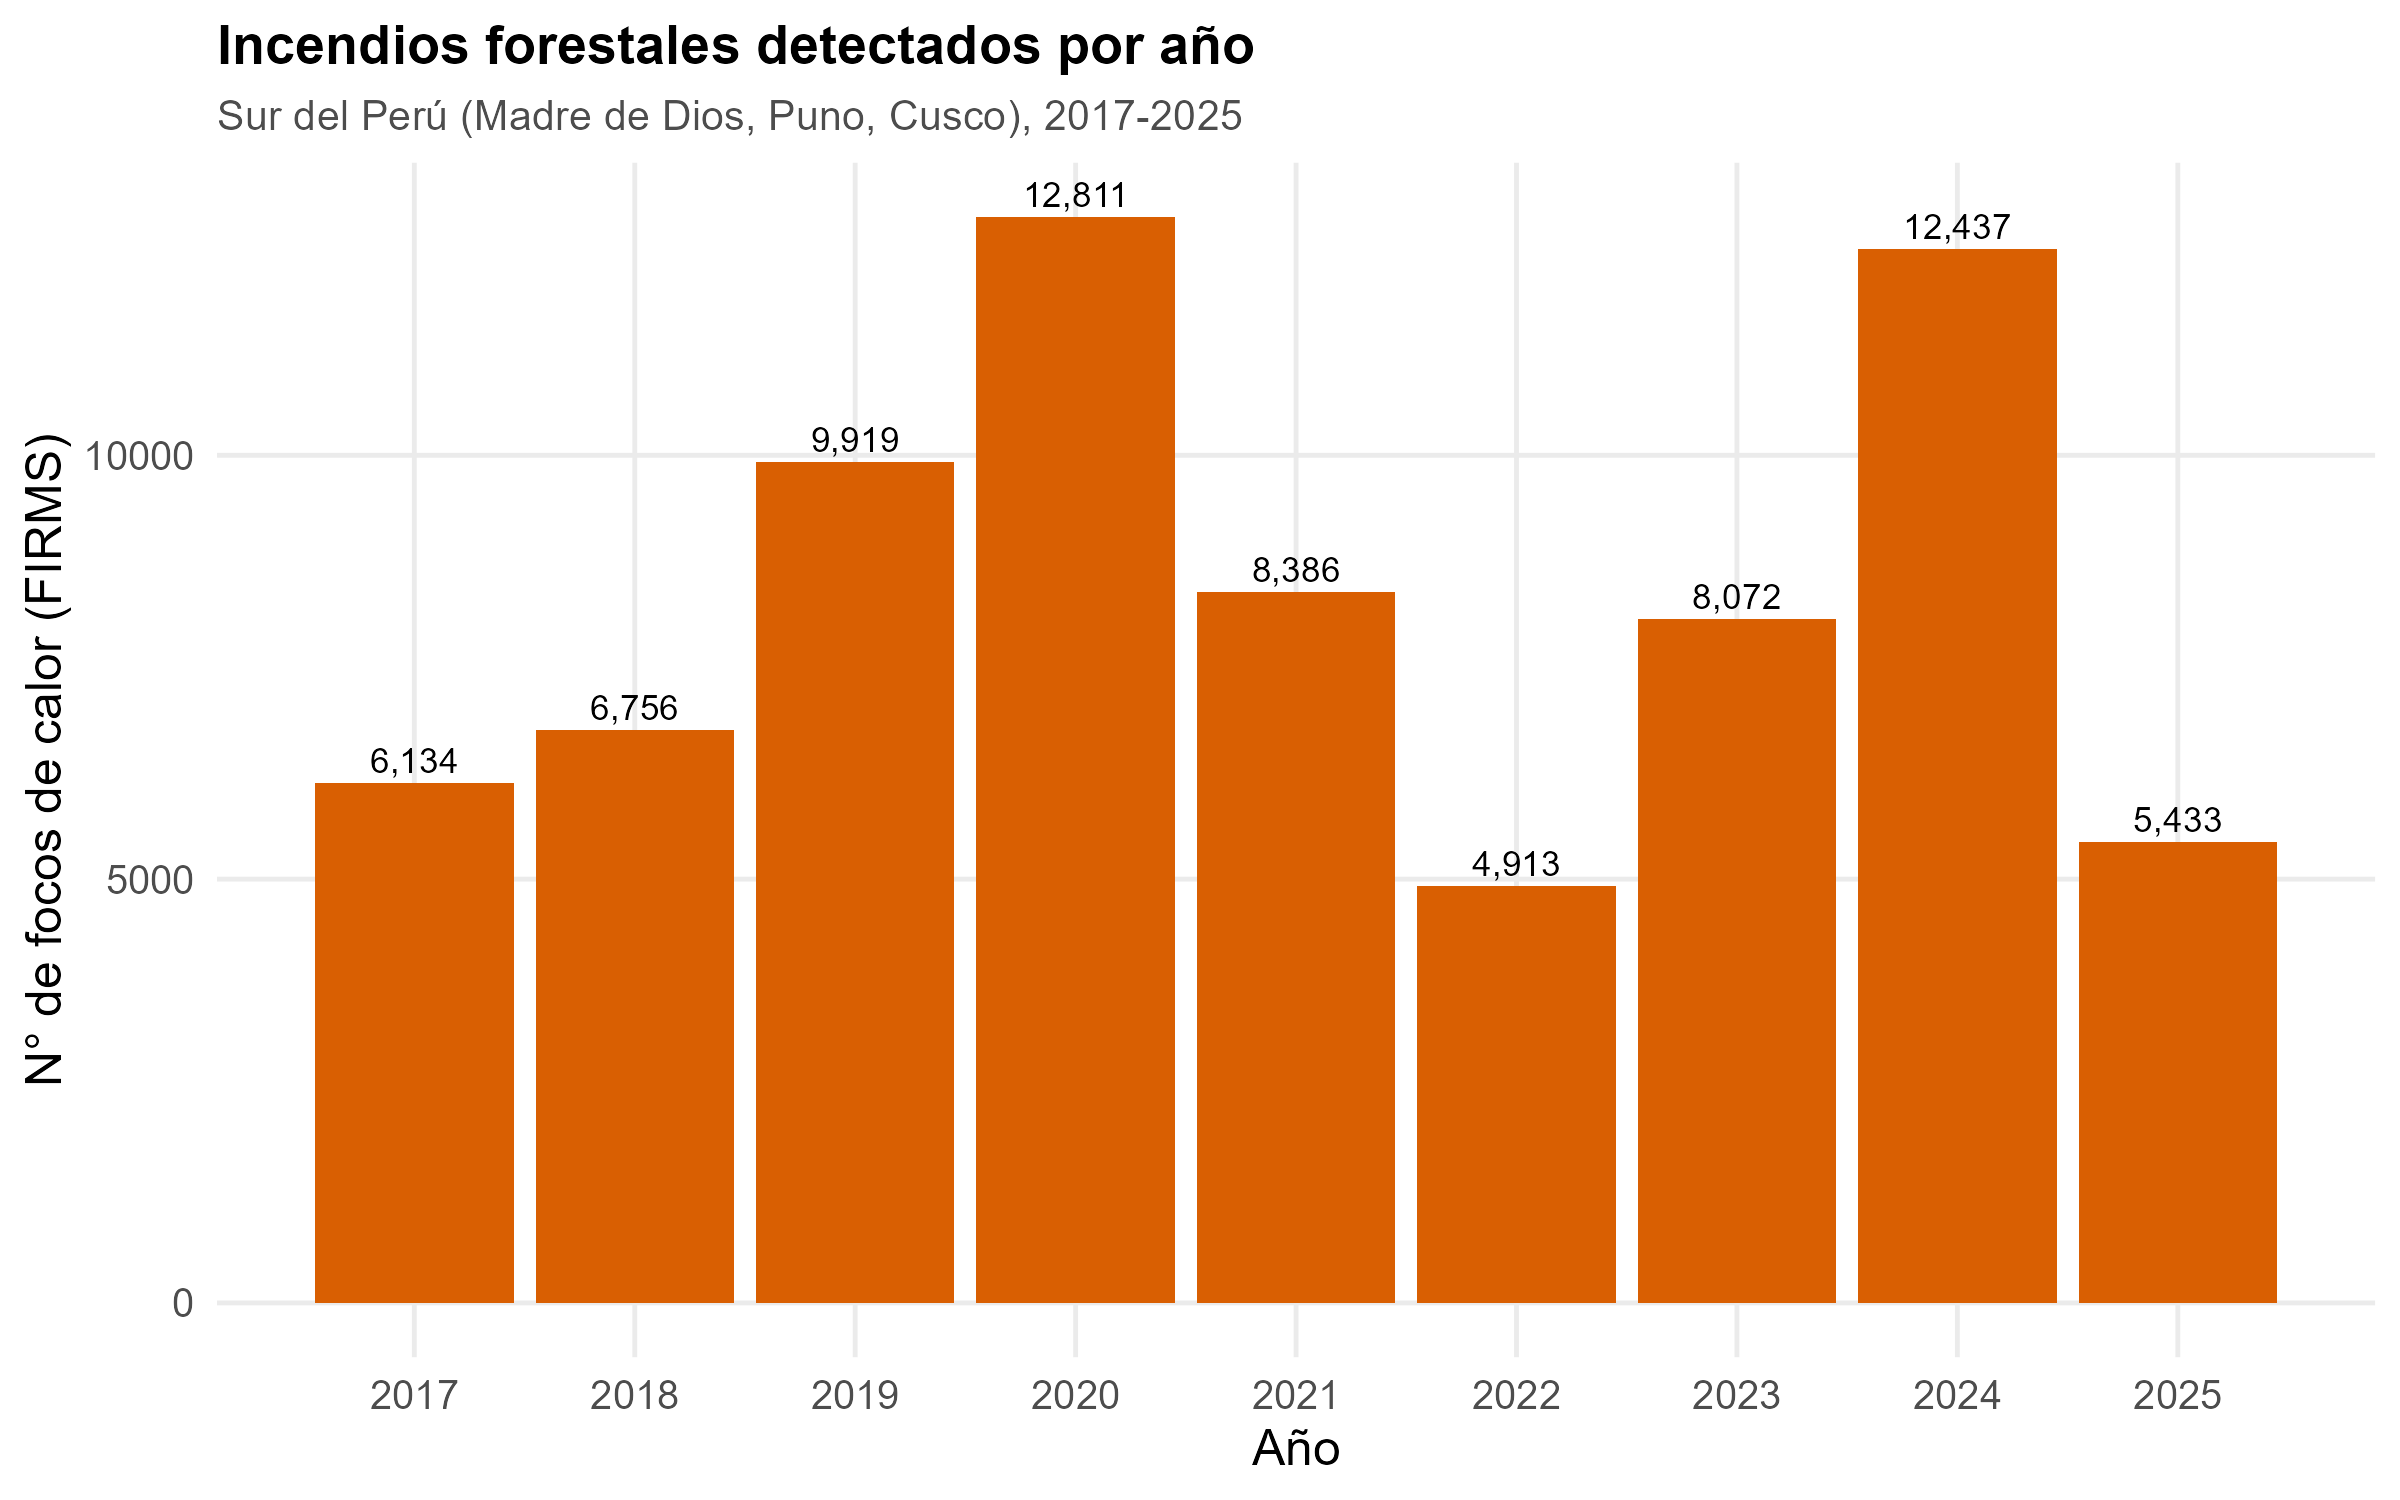
\includegraphics[width=0.88\textwidth]{serie_anual_incendios.png}
		\caption{Annual trend of forest fires in southern Peru
			(2017--2025).}
		\label{fig:serie_anual}
	\end{figure}
	
	\begin{figure}[htbp]
		\centering
		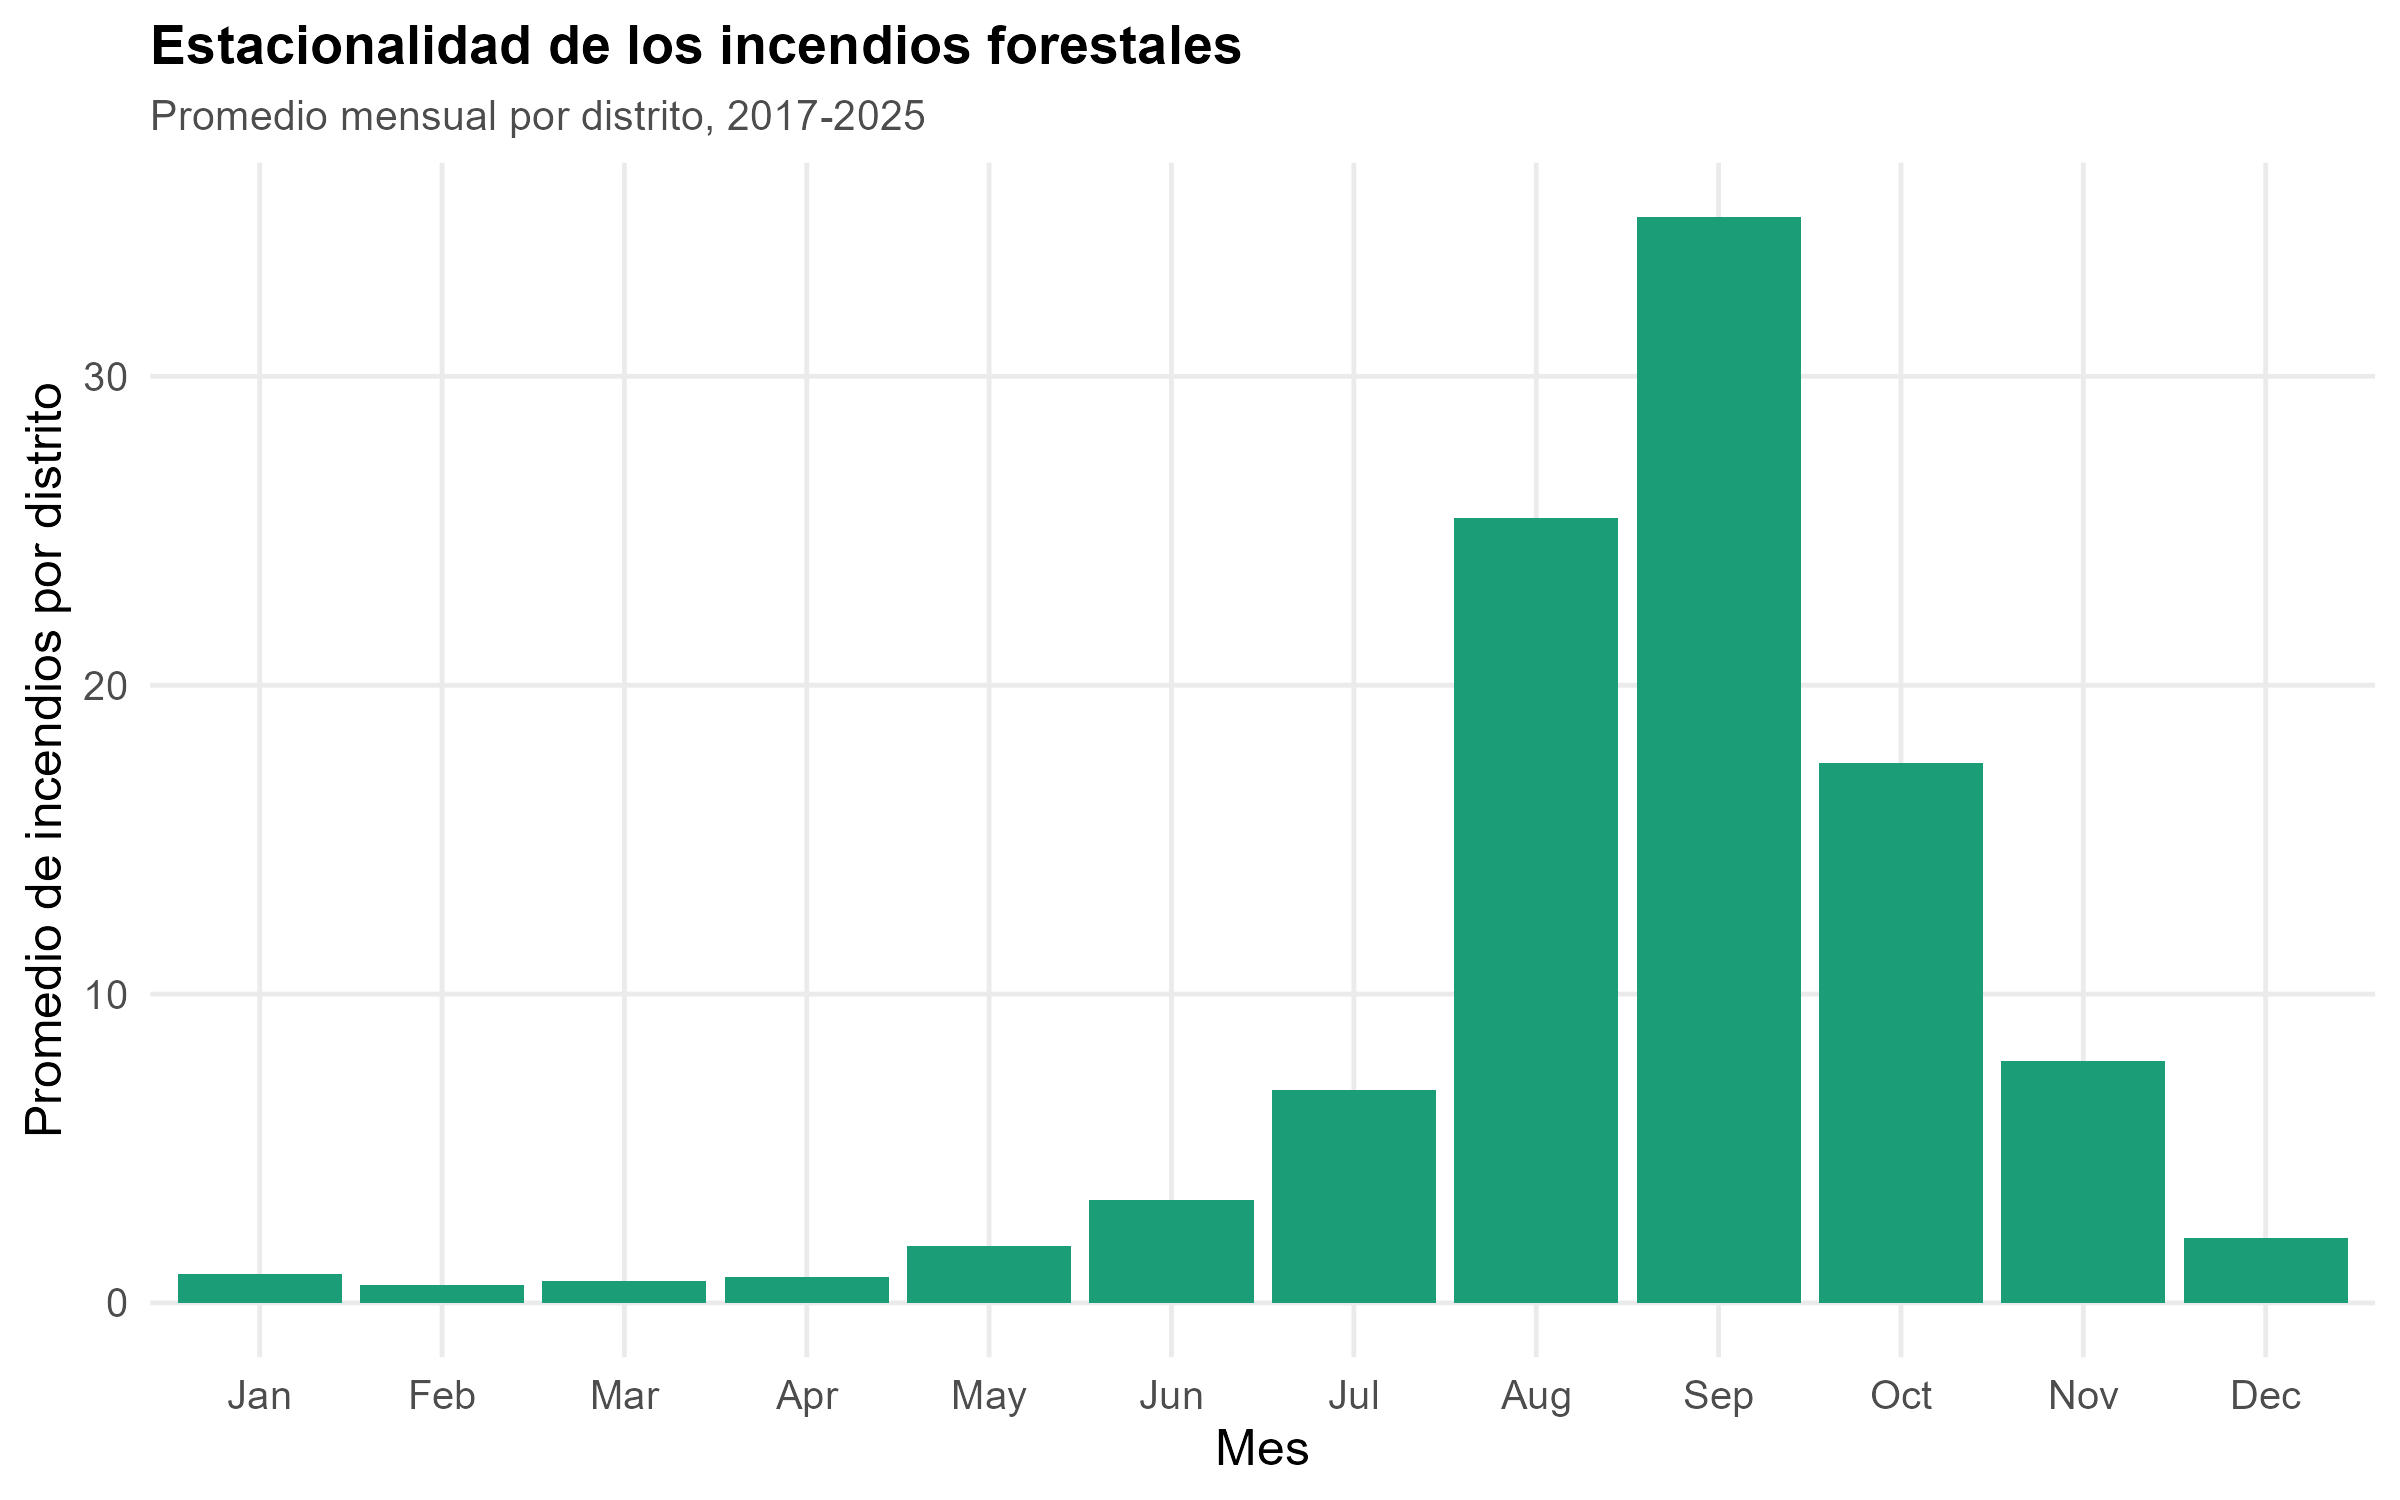
\includegraphics[width=0.88\textwidth]{estacionalidad_incendios.png}
		\caption{Aggregated monthly distribution and seasonal
			percentage of forest fires.}
		\label{fig:estacionalidad}
	\end{figure}
	
	\begin{figure}[htbp]
		\centering
		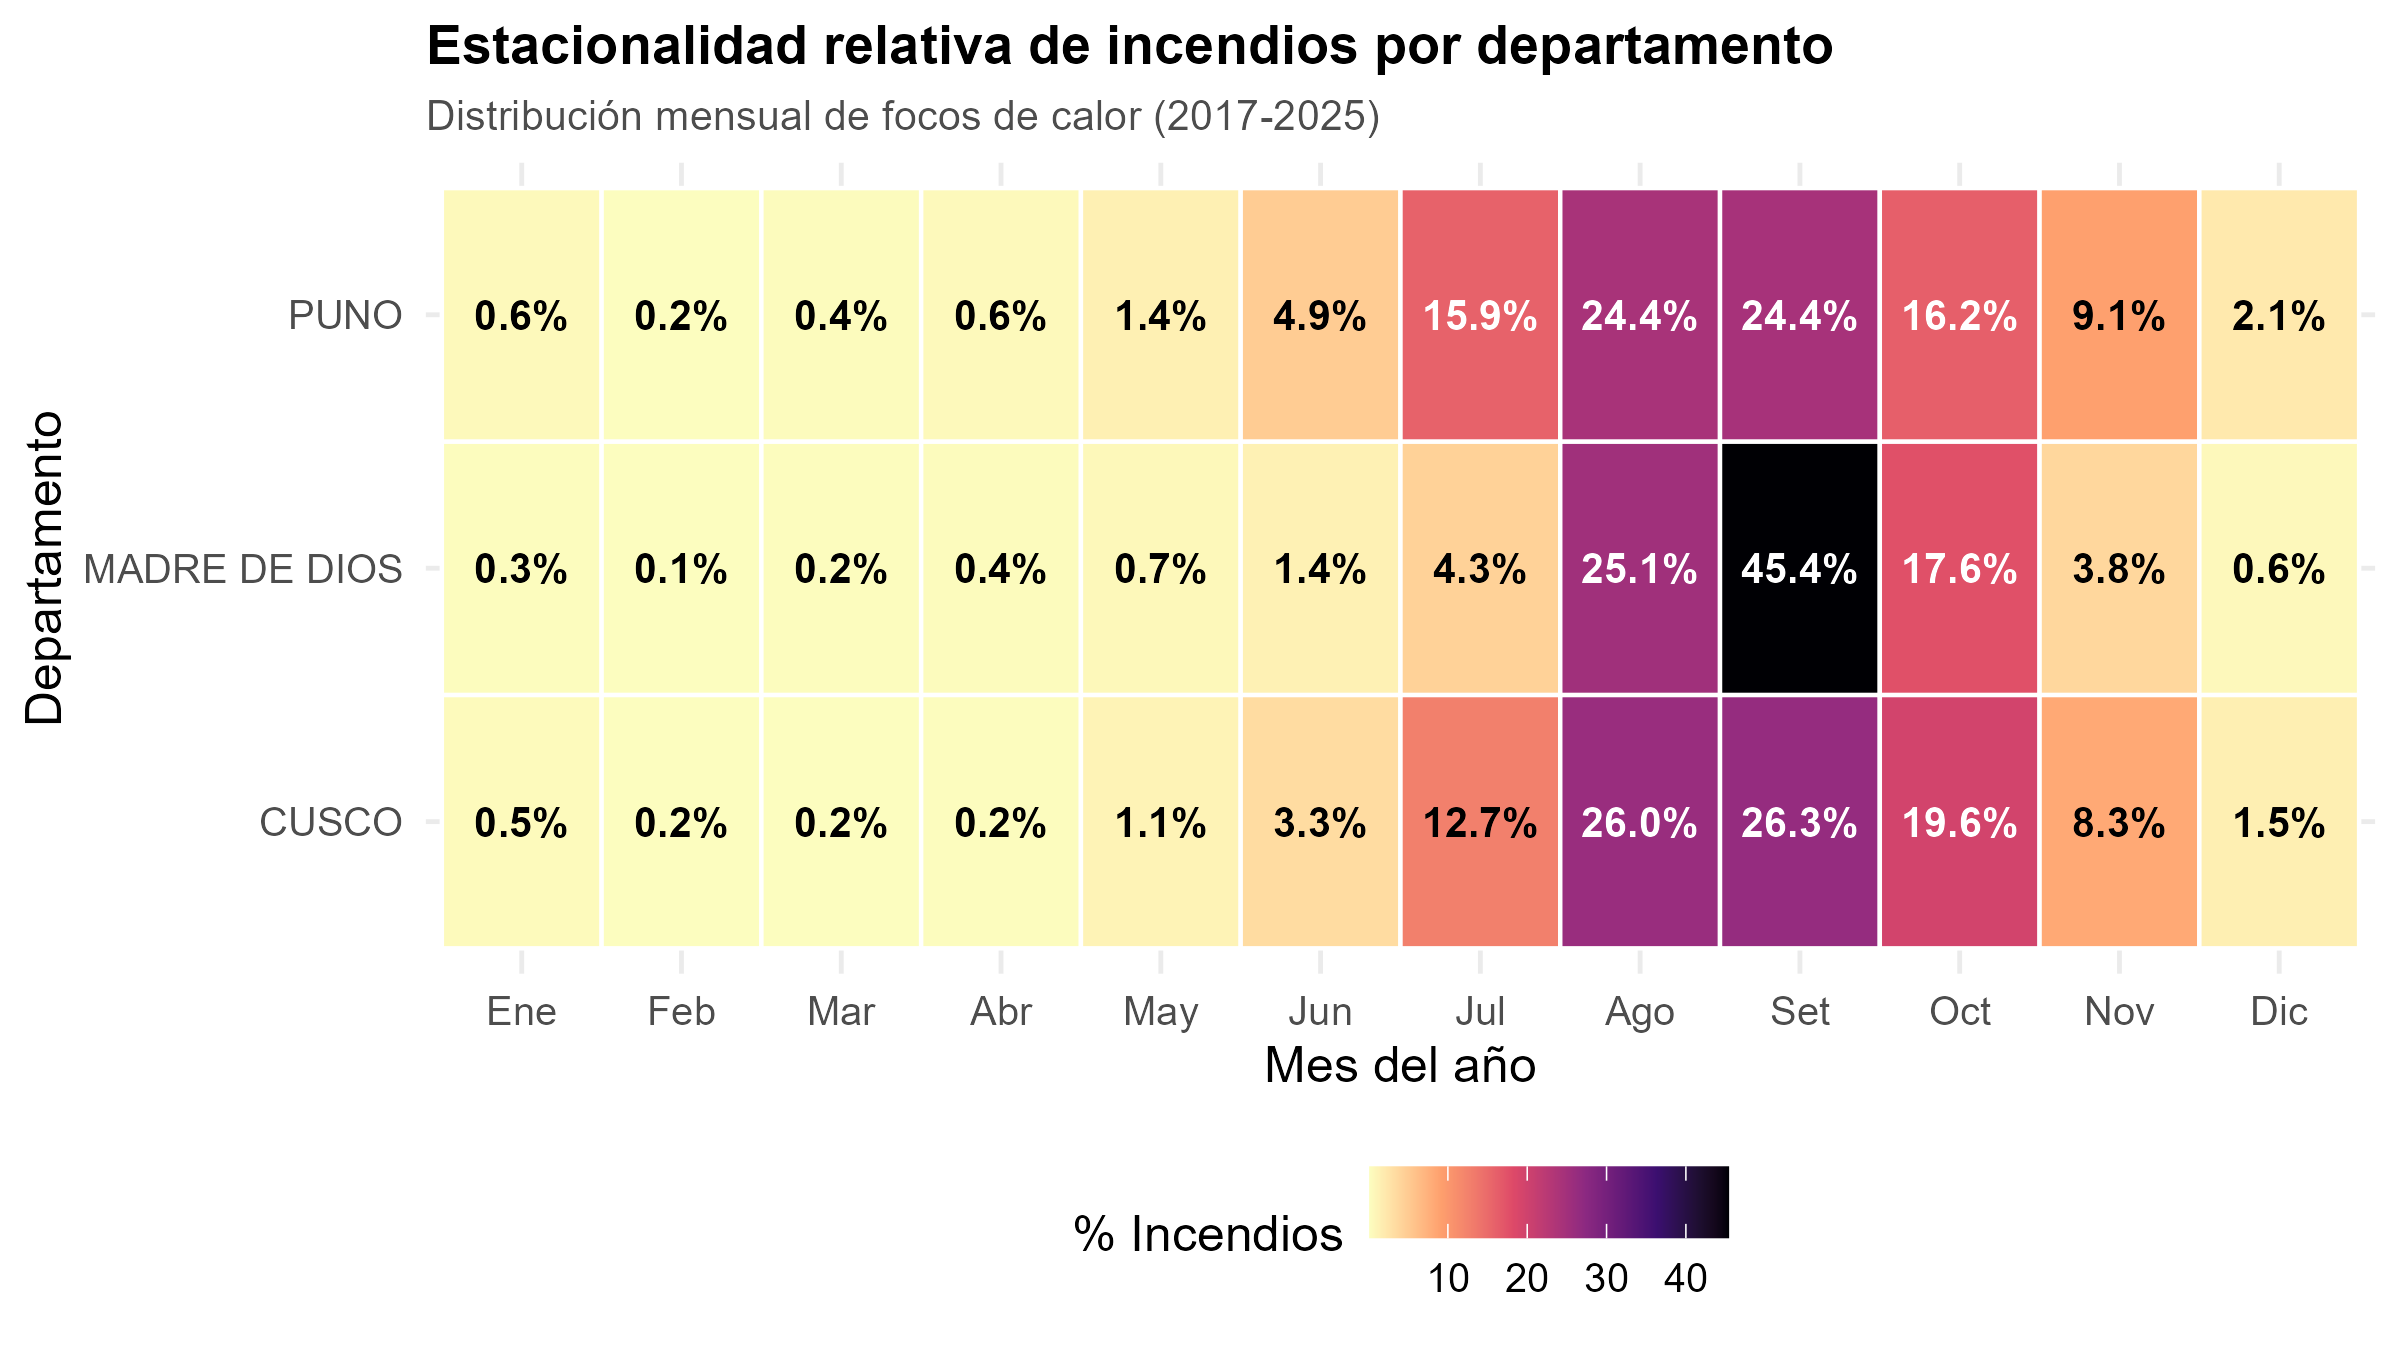
\includegraphics[width=0.92\textwidth]{heatmap_estacionalidad_departamentos.png}
		\caption{Comparative heat map of monthly seasonality by
			department (Madre de Dios, Cusco, and Puno).}
		\label{fig:heatmap}
	\end{figure}
	
	\subsection{Global Spatial Autocorrelation and LISA Maps}
	
	The Global Moran's test showed highly significant positive spatial
	autocorrelation for both forest fires ($I = 0.6407$, $z = 16.918$,
	$p < 0.00001$) and deforestation ($I = 0.5905$, $z = 15.985$,
	$p < 0.00001$). The \textbf{bivariate Moran's Index} between fires
	and prior deforestation reached $I = 0.6019$ ($p = 0.001$),
	demonstrating that forest loss in neighboring districts directly
	increases fire risk in the focal district
	(Figure~\ref{fig:moran_scatterplot}).
	
	\begin{figure}[htbp]
		\centering
		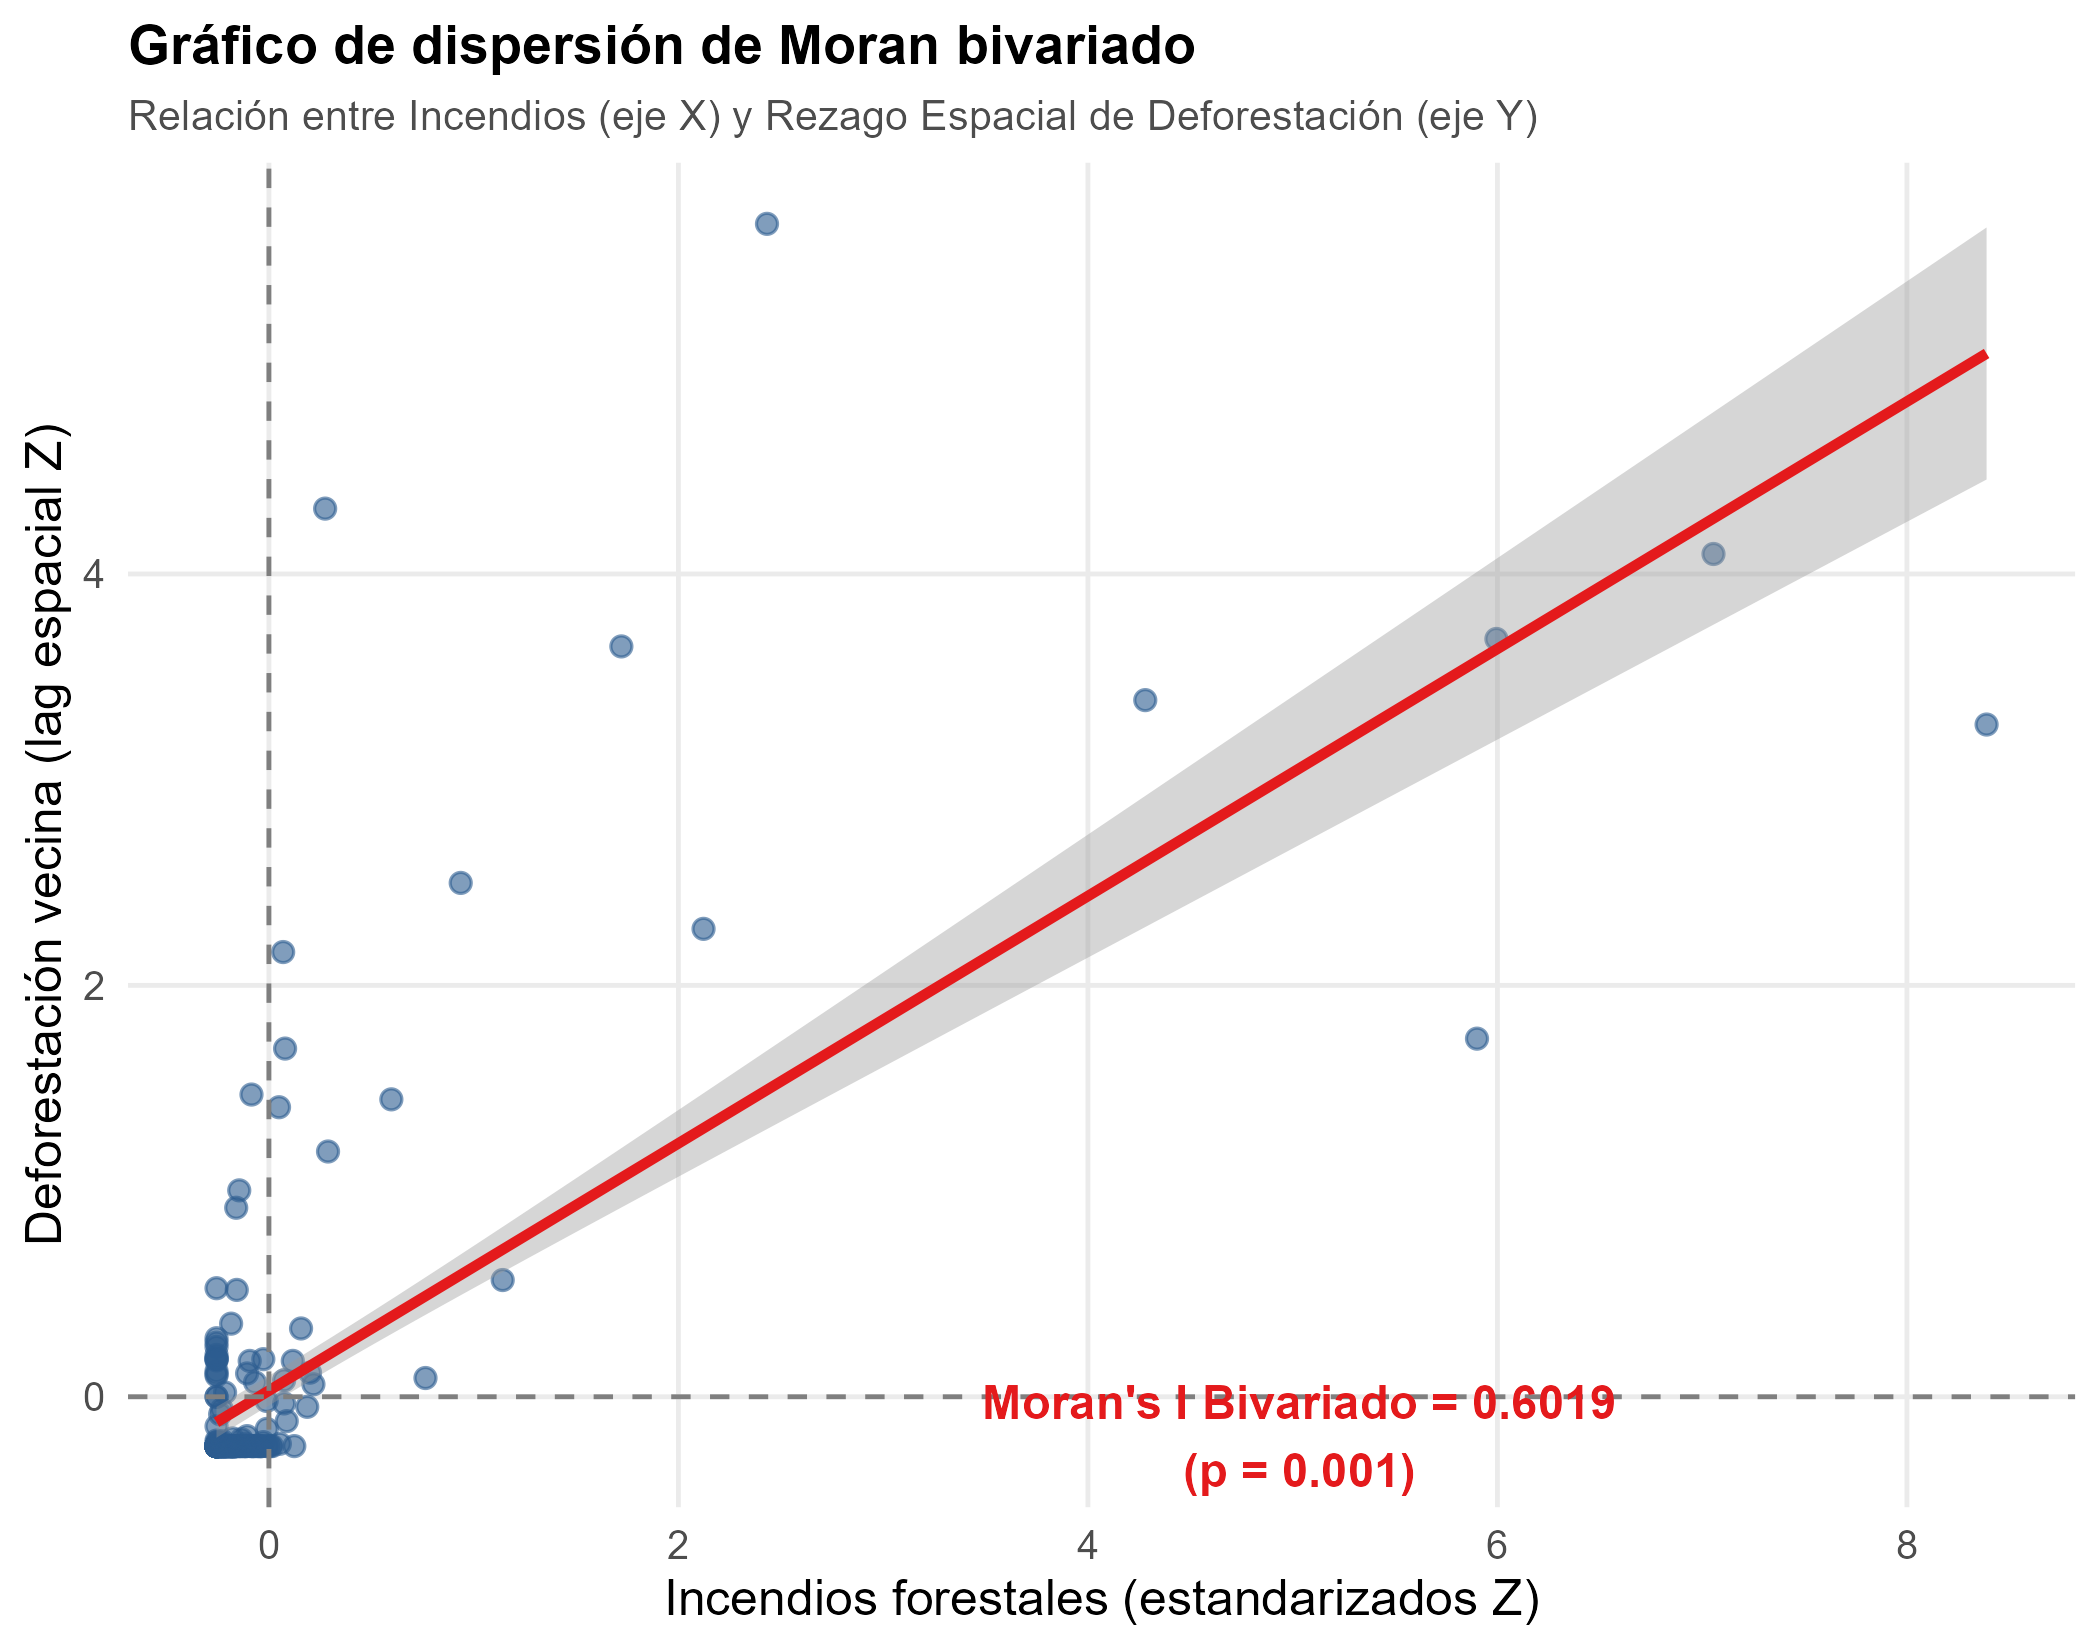
\includegraphics[width=0.78\textwidth]{moran_scatterplot_bivariado.png}
		\caption{Bivariate Moran scatterplot between fires and the
			spatial lag of deforestation ($I = 0.6019$,
			$p = 0.001$).}
		\label{fig:moran_scatterplot}
	\end{figure}
	
	The univariate (Figure~\ref{fig:lisa_univariado}) and bivariate
	(Figure~\ref{fig:lisa_bivariado}) LISA maps confirm the existence of
	statistically significant \textit{High-High} zones in northern
	Madre de Dios and at the Cusco--Puno interface, corresponding to the
	districts with the highest fire concentration and the strongest
	local association with surrounding deforestation.
	
	\begin{figure}[htbp]
		\centering
		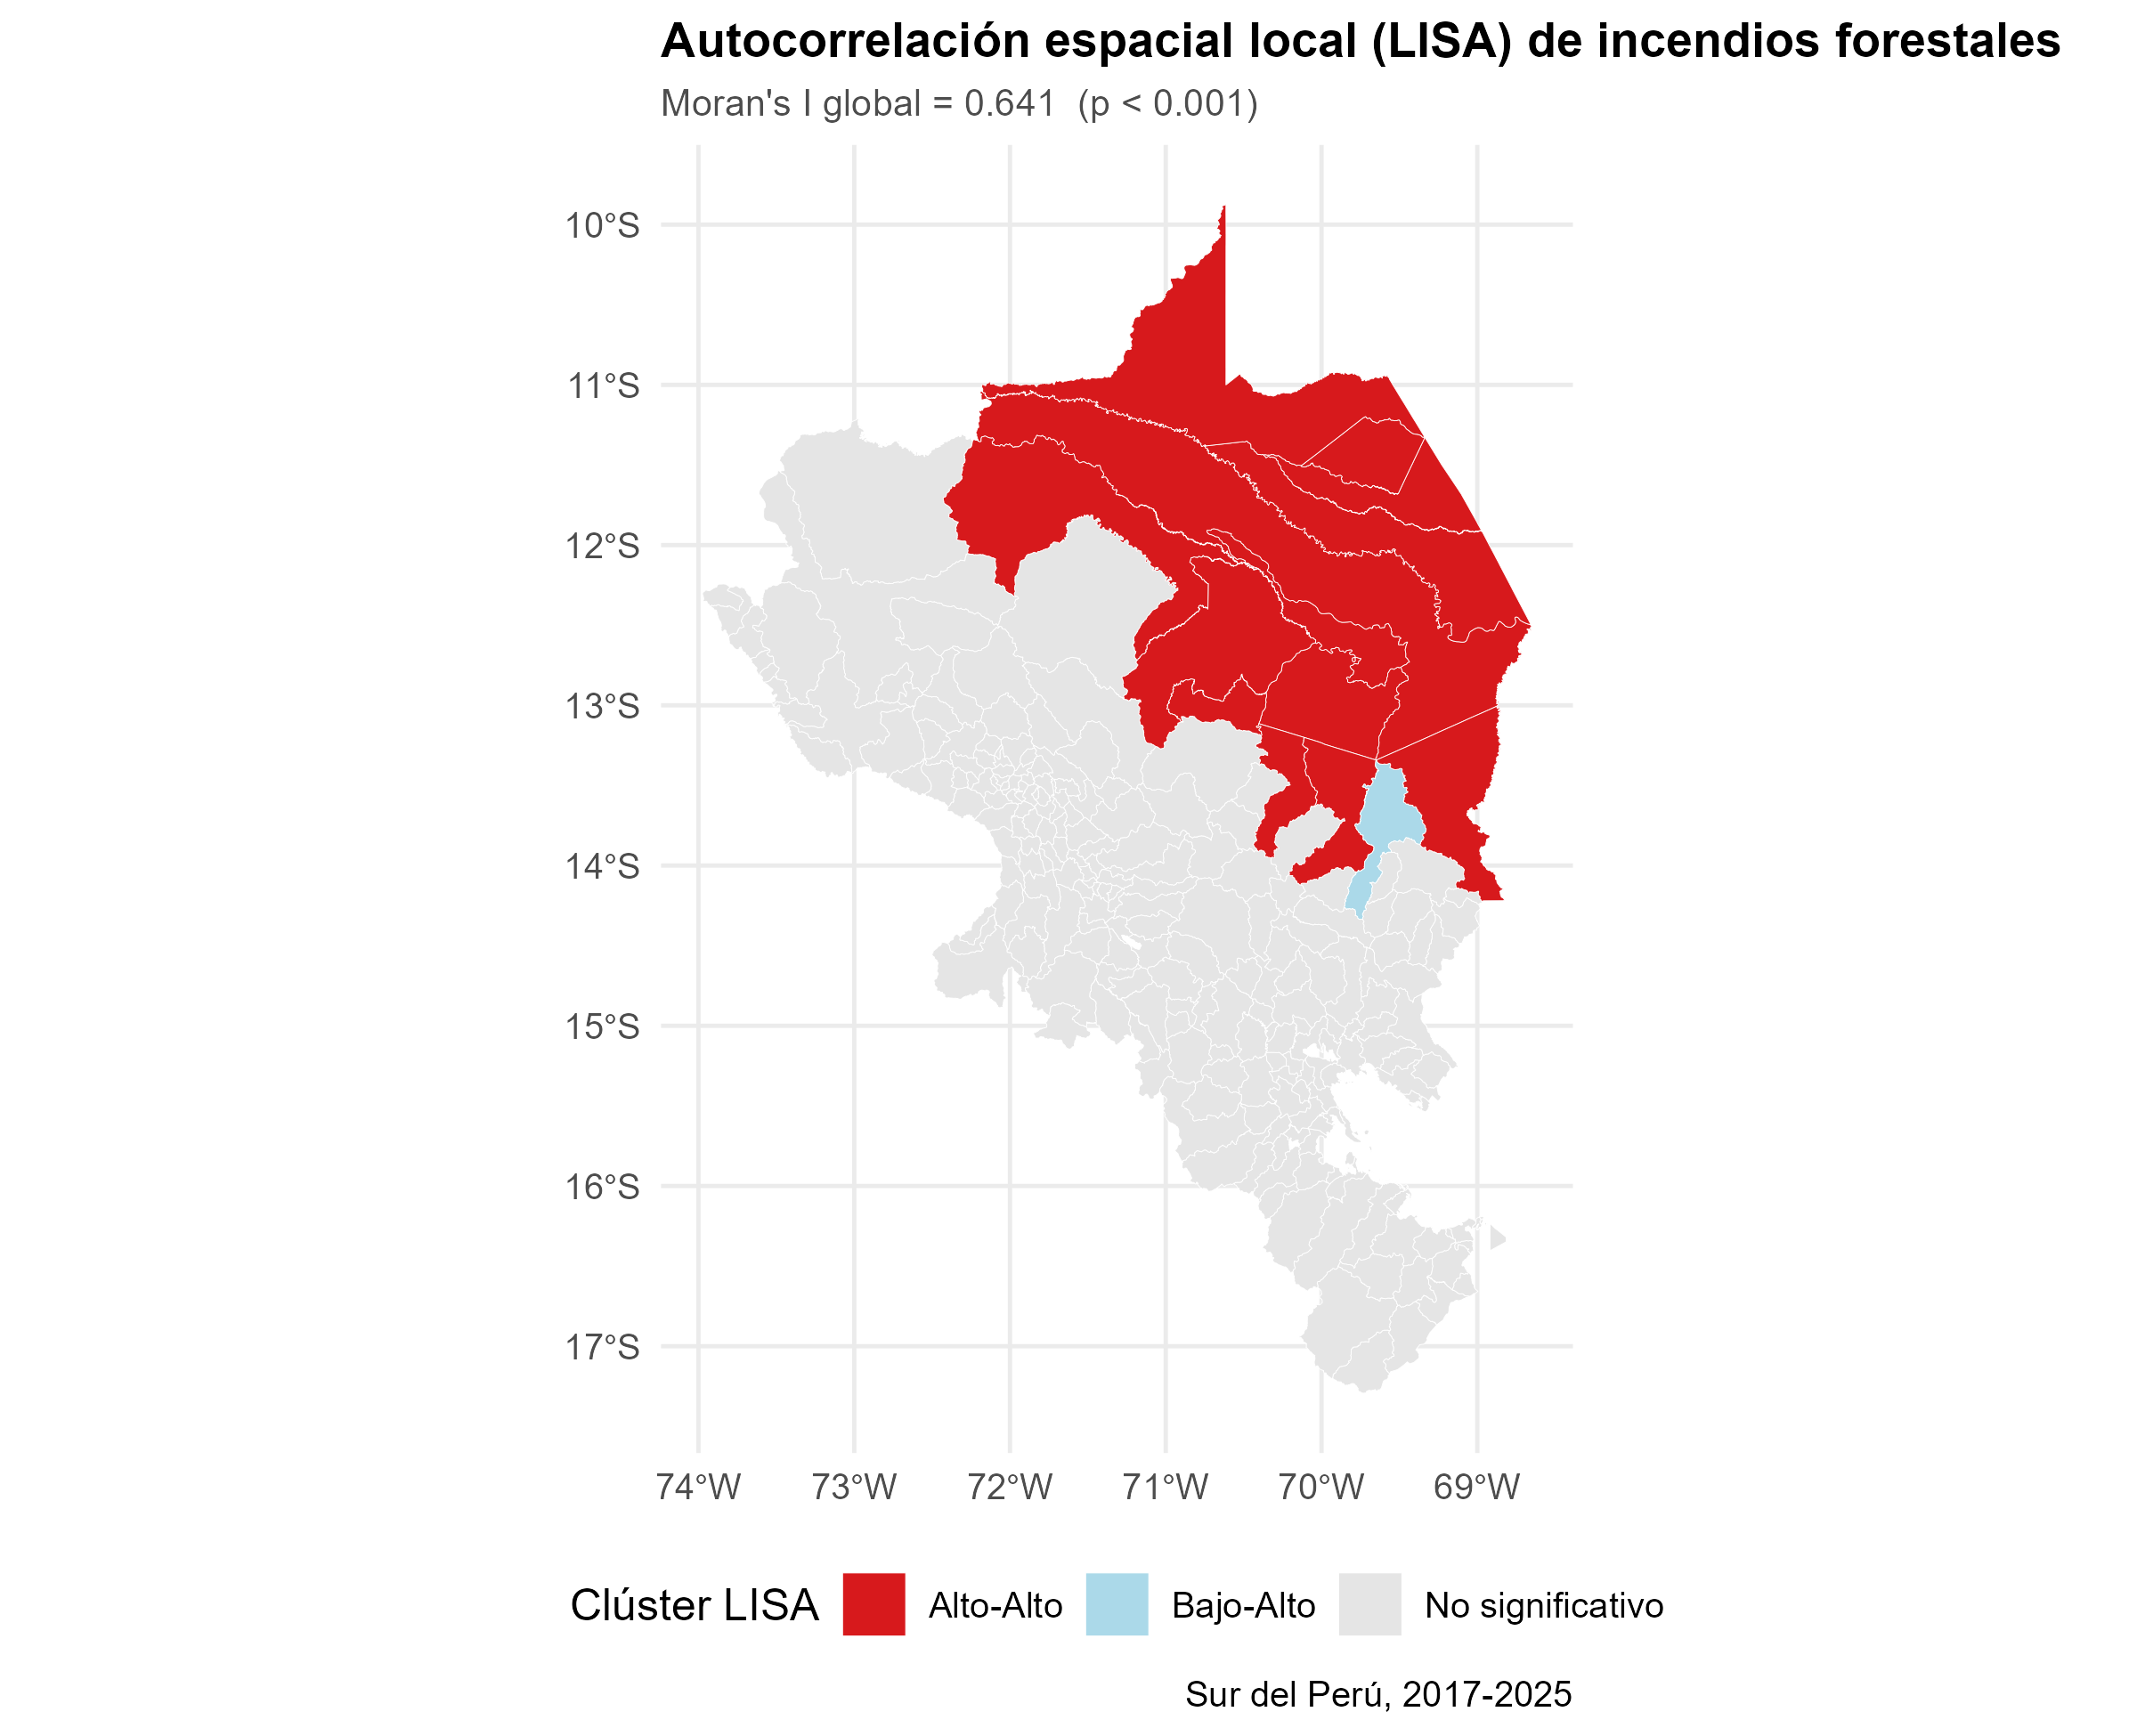
\includegraphics[width=0.85\textwidth]{lisa_incendios.png}
		\caption{Local spatial autocorrelation map (univariate LISA)
			of forest fires.}
		\label{fig:lisa_univariado}
	\end{figure}
	
	\begin{figure}[htbp]
		\centering
		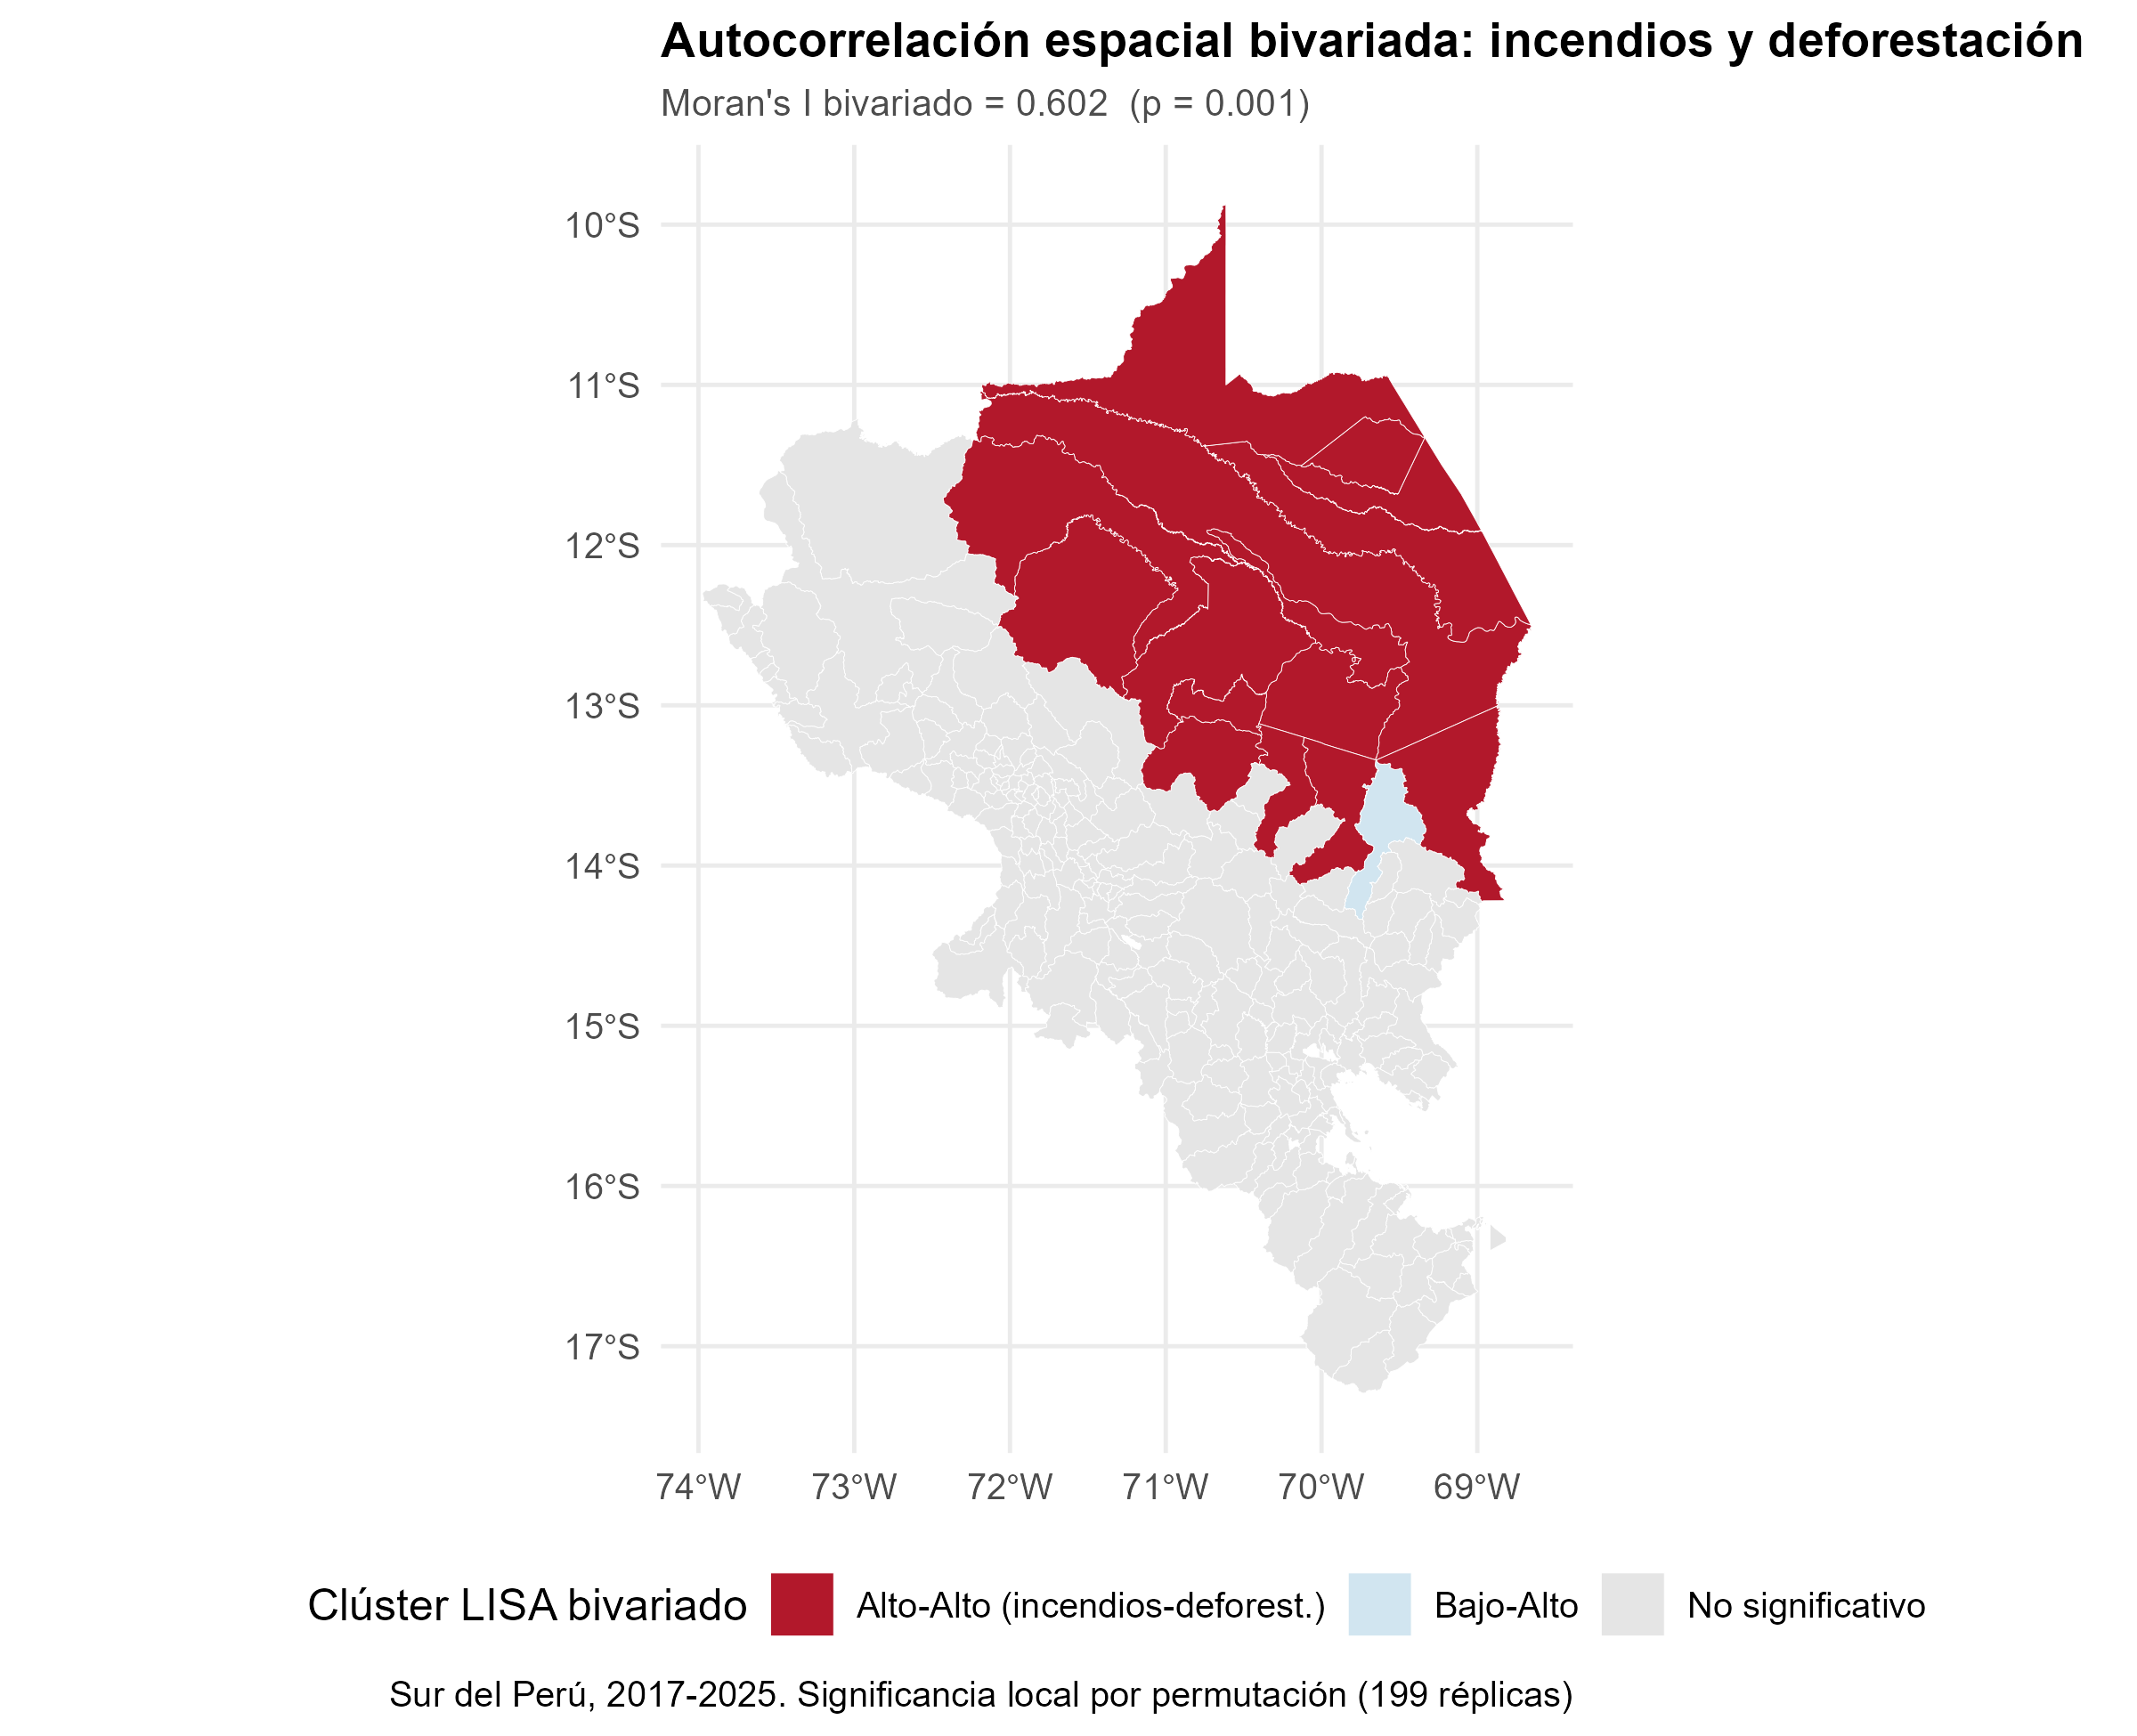
\includegraphics[width=0.85\textwidth]{lisa_bivariado_incendios_deforestacion.png}
		\caption{Bivariate LISA map: local association between
			deforestation and forest fires.}
		\label{fig:lisa_bivariado}
	\end{figure}
	
	\subsection{Spatio-Temporal Cluster Detection (SaTScan)}
	
	\textbf{Nine statistically significant spatio-temporal clusters}
	were identified ($p < 0.00001$), detailed in
	Table~\ref{tab:clusters} and mapped in
	Figure~\ref{fig:mapa_clusters}. The active temporal window of each
	cluster is shown in Figure~\ref{fig:gantt}.
	
	\begin{table}[H]
		\centering
		\caption{Spatio-temporal forest-fire clusters detected using SaTScan}
		\label{tab:clusters}
		\begin{tabular}{ccccccc}
			\toprule
			Cluster & Districts & Period & Radius (km) & Observed & RR & LLR \\
			\midrule
			1 & 96 & 2019/1/1 - 2022-12-31 & 143.9 & 6273 & 780.02 & 35231.2 \\
			2 & 130 & 2024/1/1 - 2024-12-31 & 178.1 & 1059 & 293.30 & 4953.5 \\
			3 & 47 & 2019/1/1 - 2022-12-31 & 86.9 & 1263 & 42.48 & 3491.5 \\
			4 & 5 & 2023/1/1 - 2025-12-31 & 81.5 & 14264 & 2.16 & 2908.3 \\
			5 & 95 & 2017/1/1 - 2017-12-31 & 143.5 & 482 & 296.55 & 2261.7 \\
			6 & 4 & 2018/1/1 - 2021-12-31 & 95.1 & 15863 & 1.80 & 1933.3 \\
			7 & 2 & 2019/1/1 - 2022-12-31 & 31.4 & 378 & 11.84 & 587.5 \\
			8 & 5 & 2018/1/1 - 2020-12-31 & 90.6 & 2064 & 2.26 & 521.4 \\
			9 & 21 & 2017/1/1 - 2017-12-31 & 54.5 & 67 & 184.67 & 283.0 \\
			\bottomrule
		\end{tabular}
	\end{table}
	
	\begin{figure}[htbp]
		\centering
		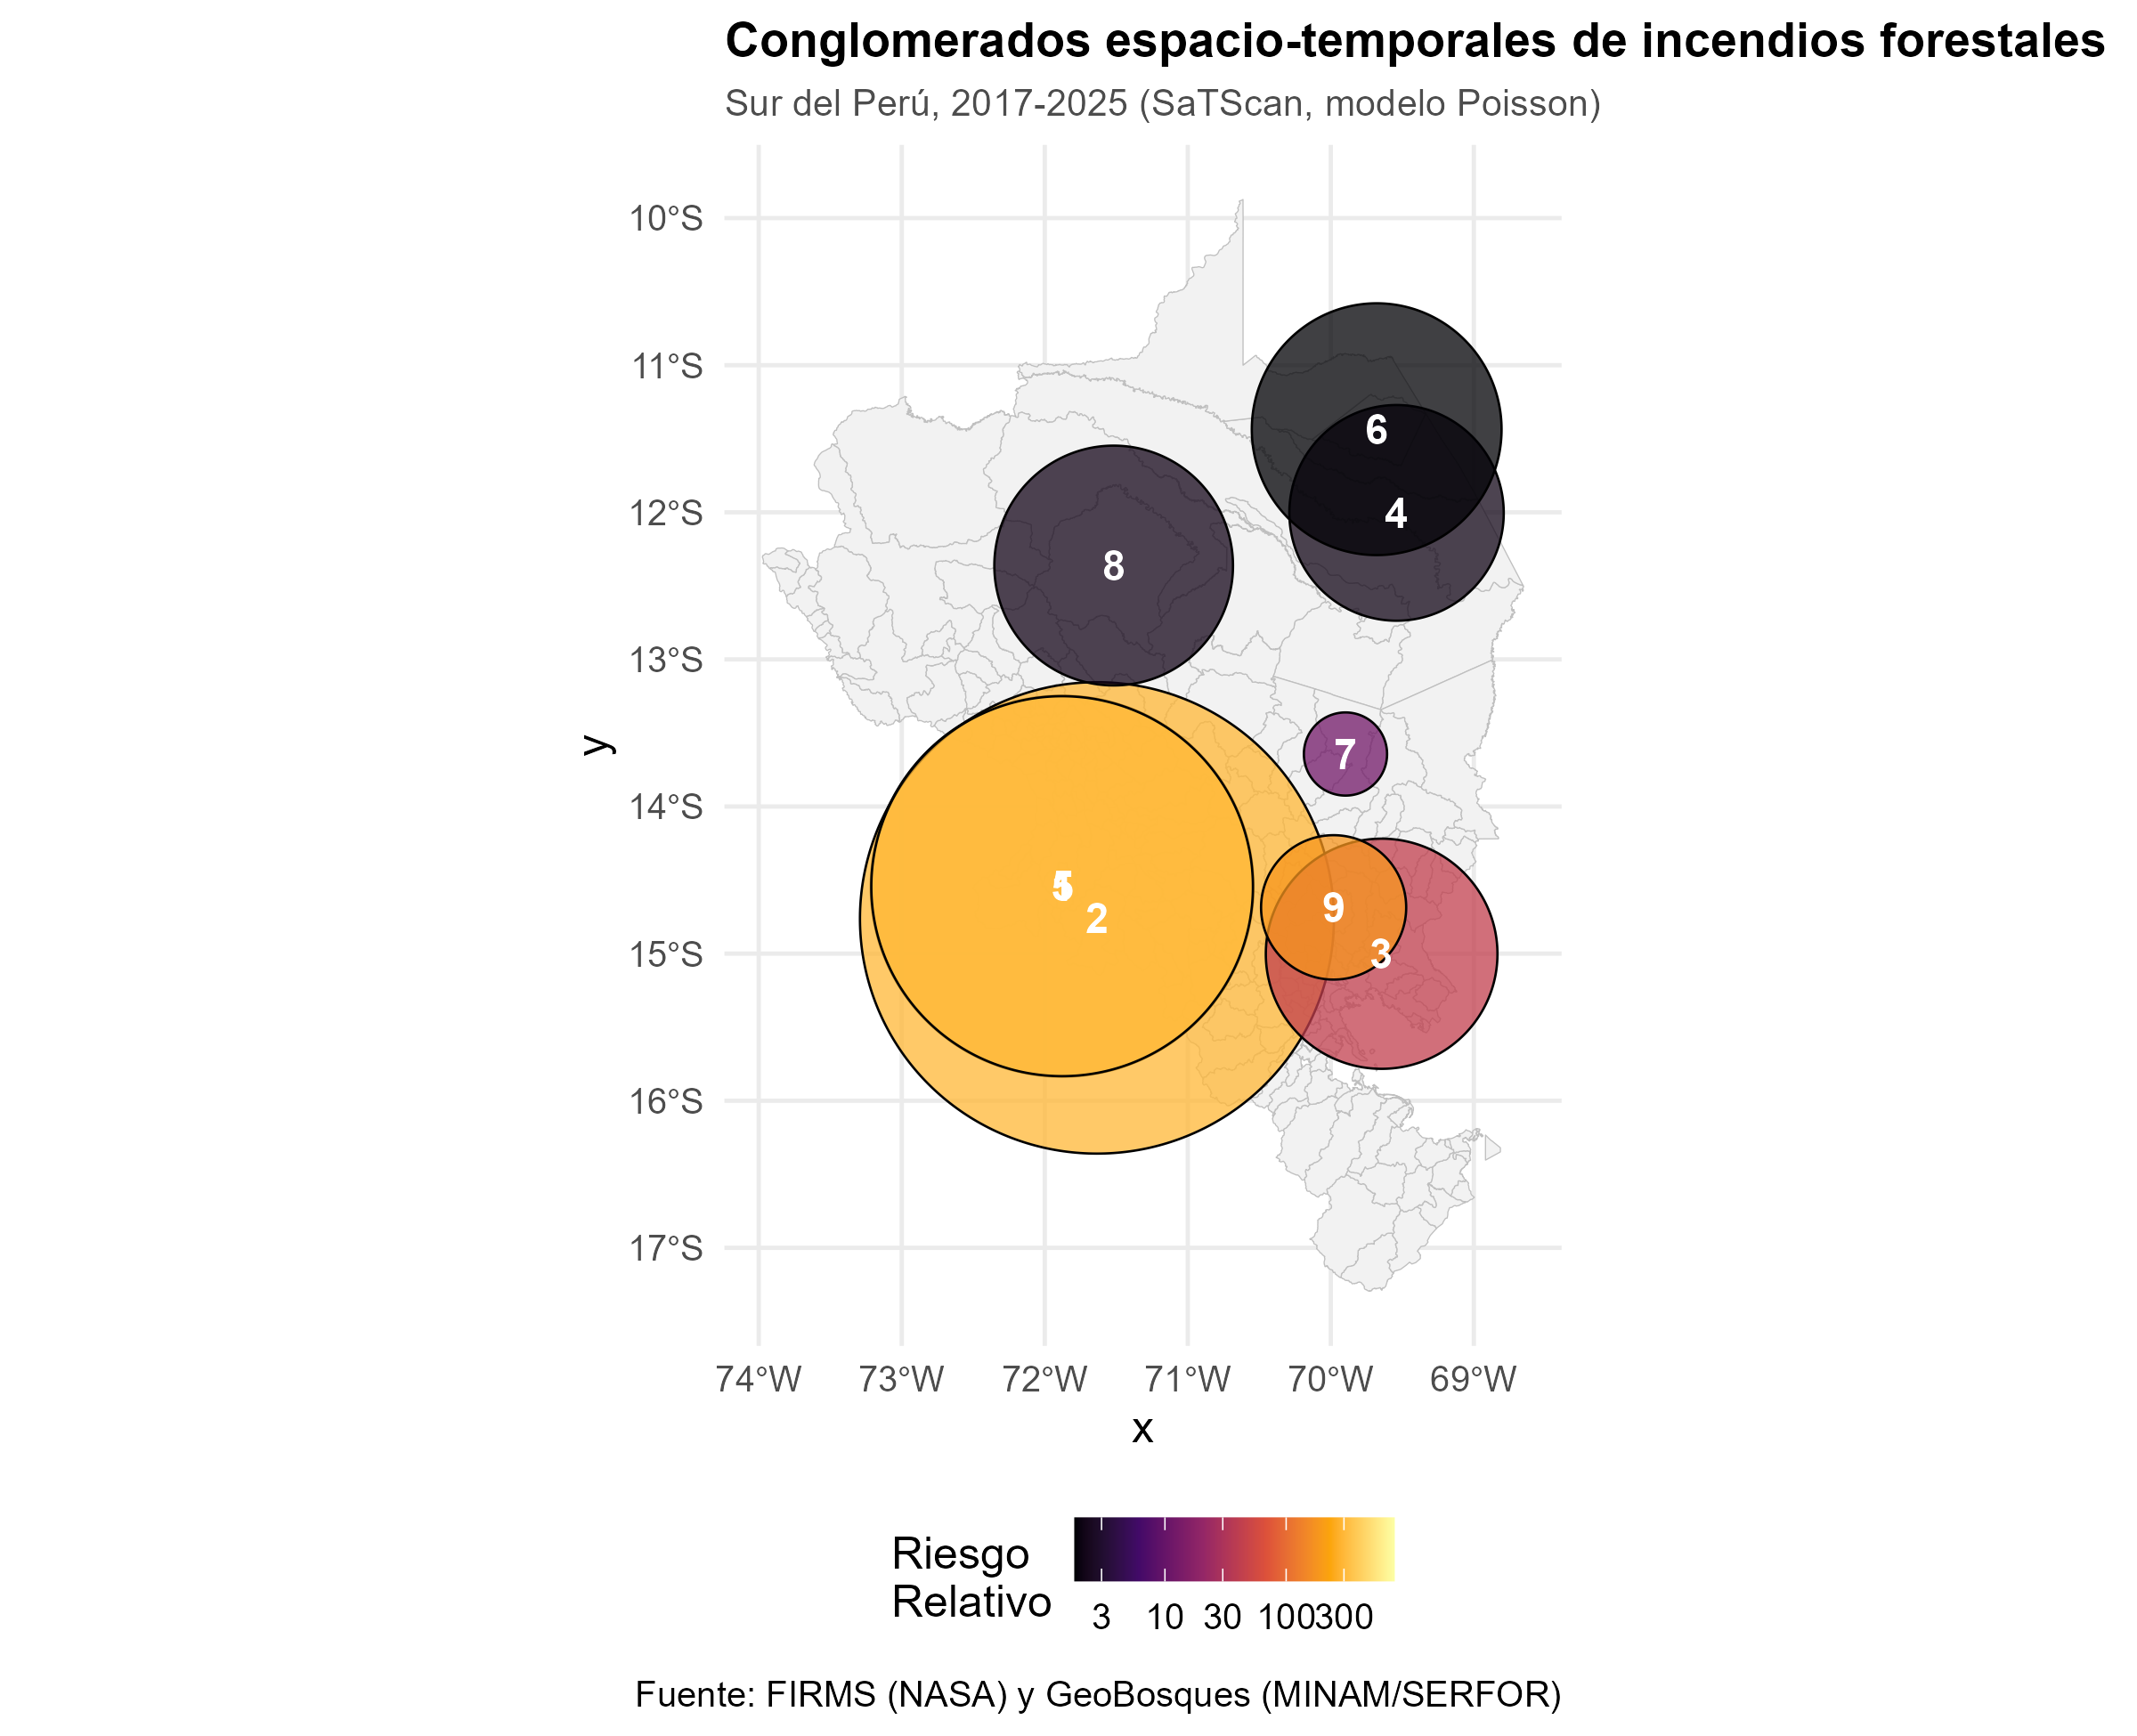
\includegraphics[width=0.88\textwidth]{mapa_clusters_etiquetado.png}
		\caption{Map of spatio-temporal forest-fire clusters detected
			by SaTScan (2017--2025).}
		\label{fig:mapa_clusters}
	\end{figure}
	
	\begin{figure}[htbp]
		\centering
		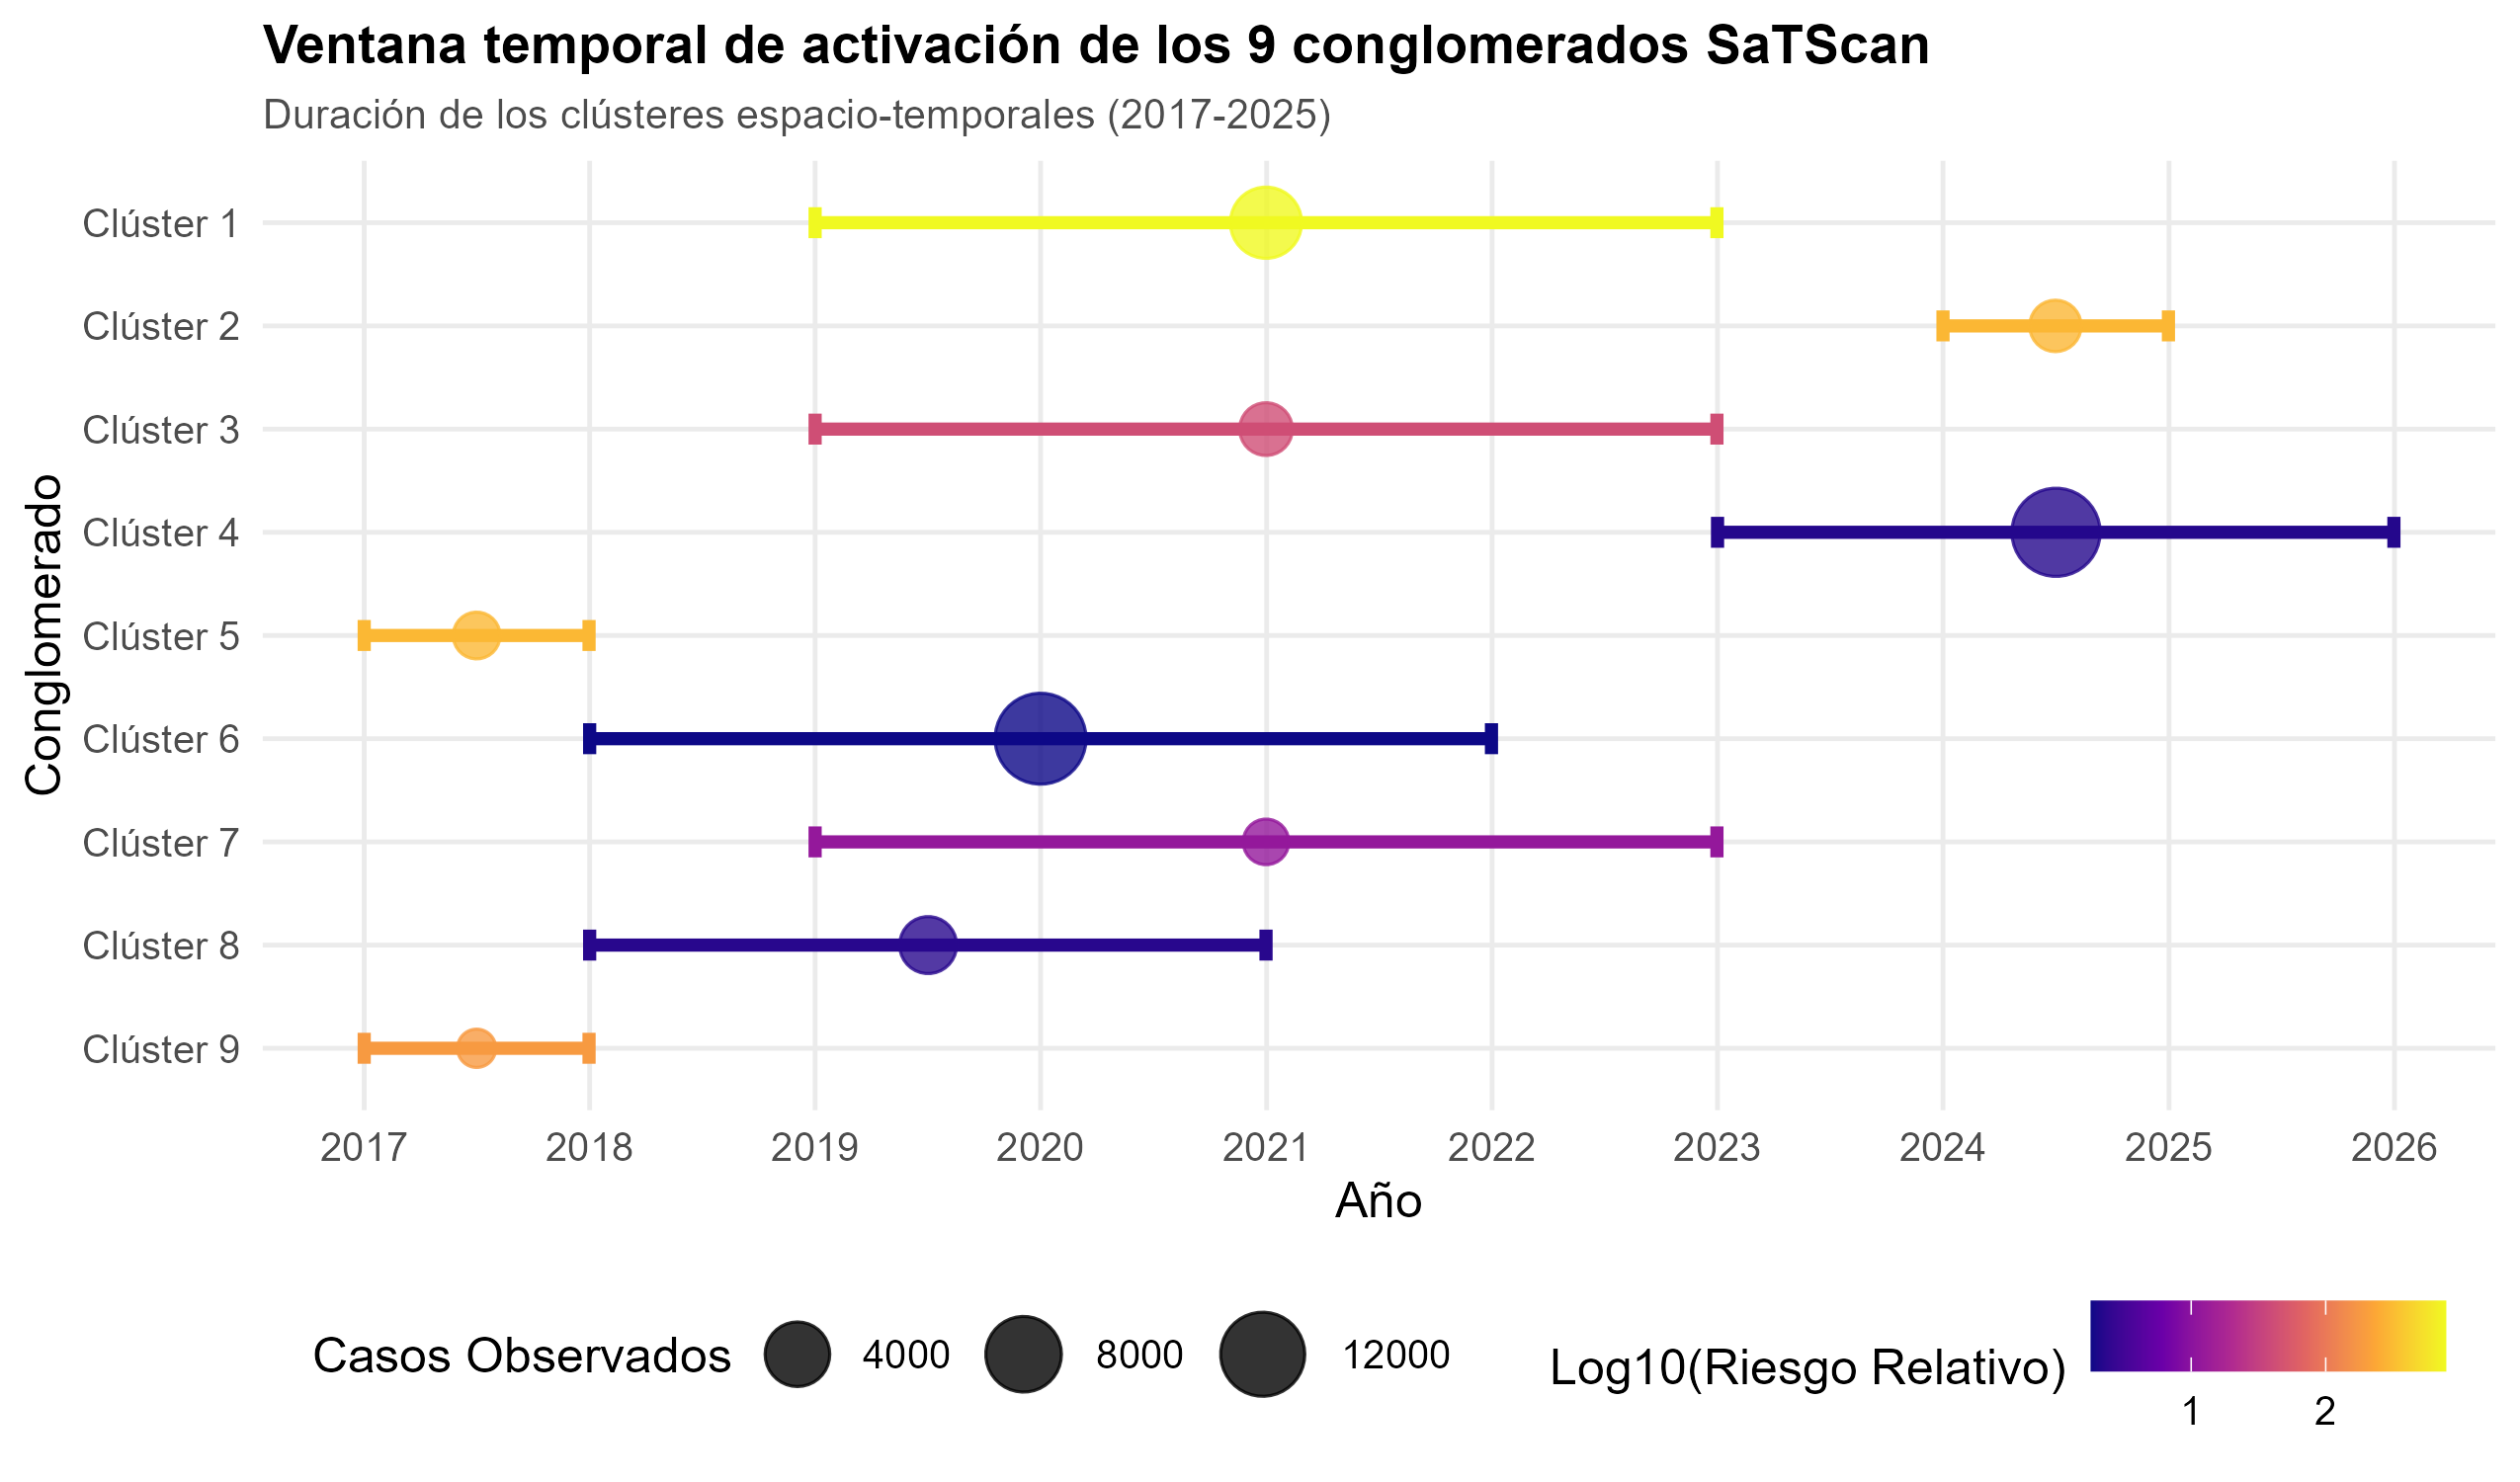
\includegraphics[width=0.92\textwidth]{linea_tiempo_clusters.png}
		\caption{Gantt chart of the active temporal window of the
			9 SaTScan clusters.}
		\label{fig:gantt}
	\end{figure}
	
	\textbf{Cluster~1 (Primary)} spans 96 districts at the Cusco--Puno
	Andean interface (period 2019--2022, radius 143.9~km), standing out
	for the highest log-likelihood ratio statistic
	($\text{LLR} = 35{,}231.2$) and a \textbf{Relative Risk of 780.02}
	(6{,}273 observed cases versus 8.8 expected).
	
	\textbf{Cluster~2} groups 130 districts in high-Andean areas of
	Cusco and Puno during \textbf{2024} ($\text{RR} = 293.30$),
	reflecting the wave of fires associated with that year's extreme
	drought (Figure~\ref{fig:riesgo_relativo}).
	
	Meanwhile, \textbf{Clusters~4 and 6}, in the Amazonian department of
	Madre de Dios, register the highest absolute burdens: Cluster~4
	(5 districts, 2023--2025) totaled \textbf{14{,}264 fires}
	($\text{RR} = 2.16$), while Cluster~6 (4 districts, 2018--2021)
	accumulated \textbf{15{,}863 fires} ($\text{RR} = 1.80$).
	
	\begin{figure}[htbp]
		\centering
		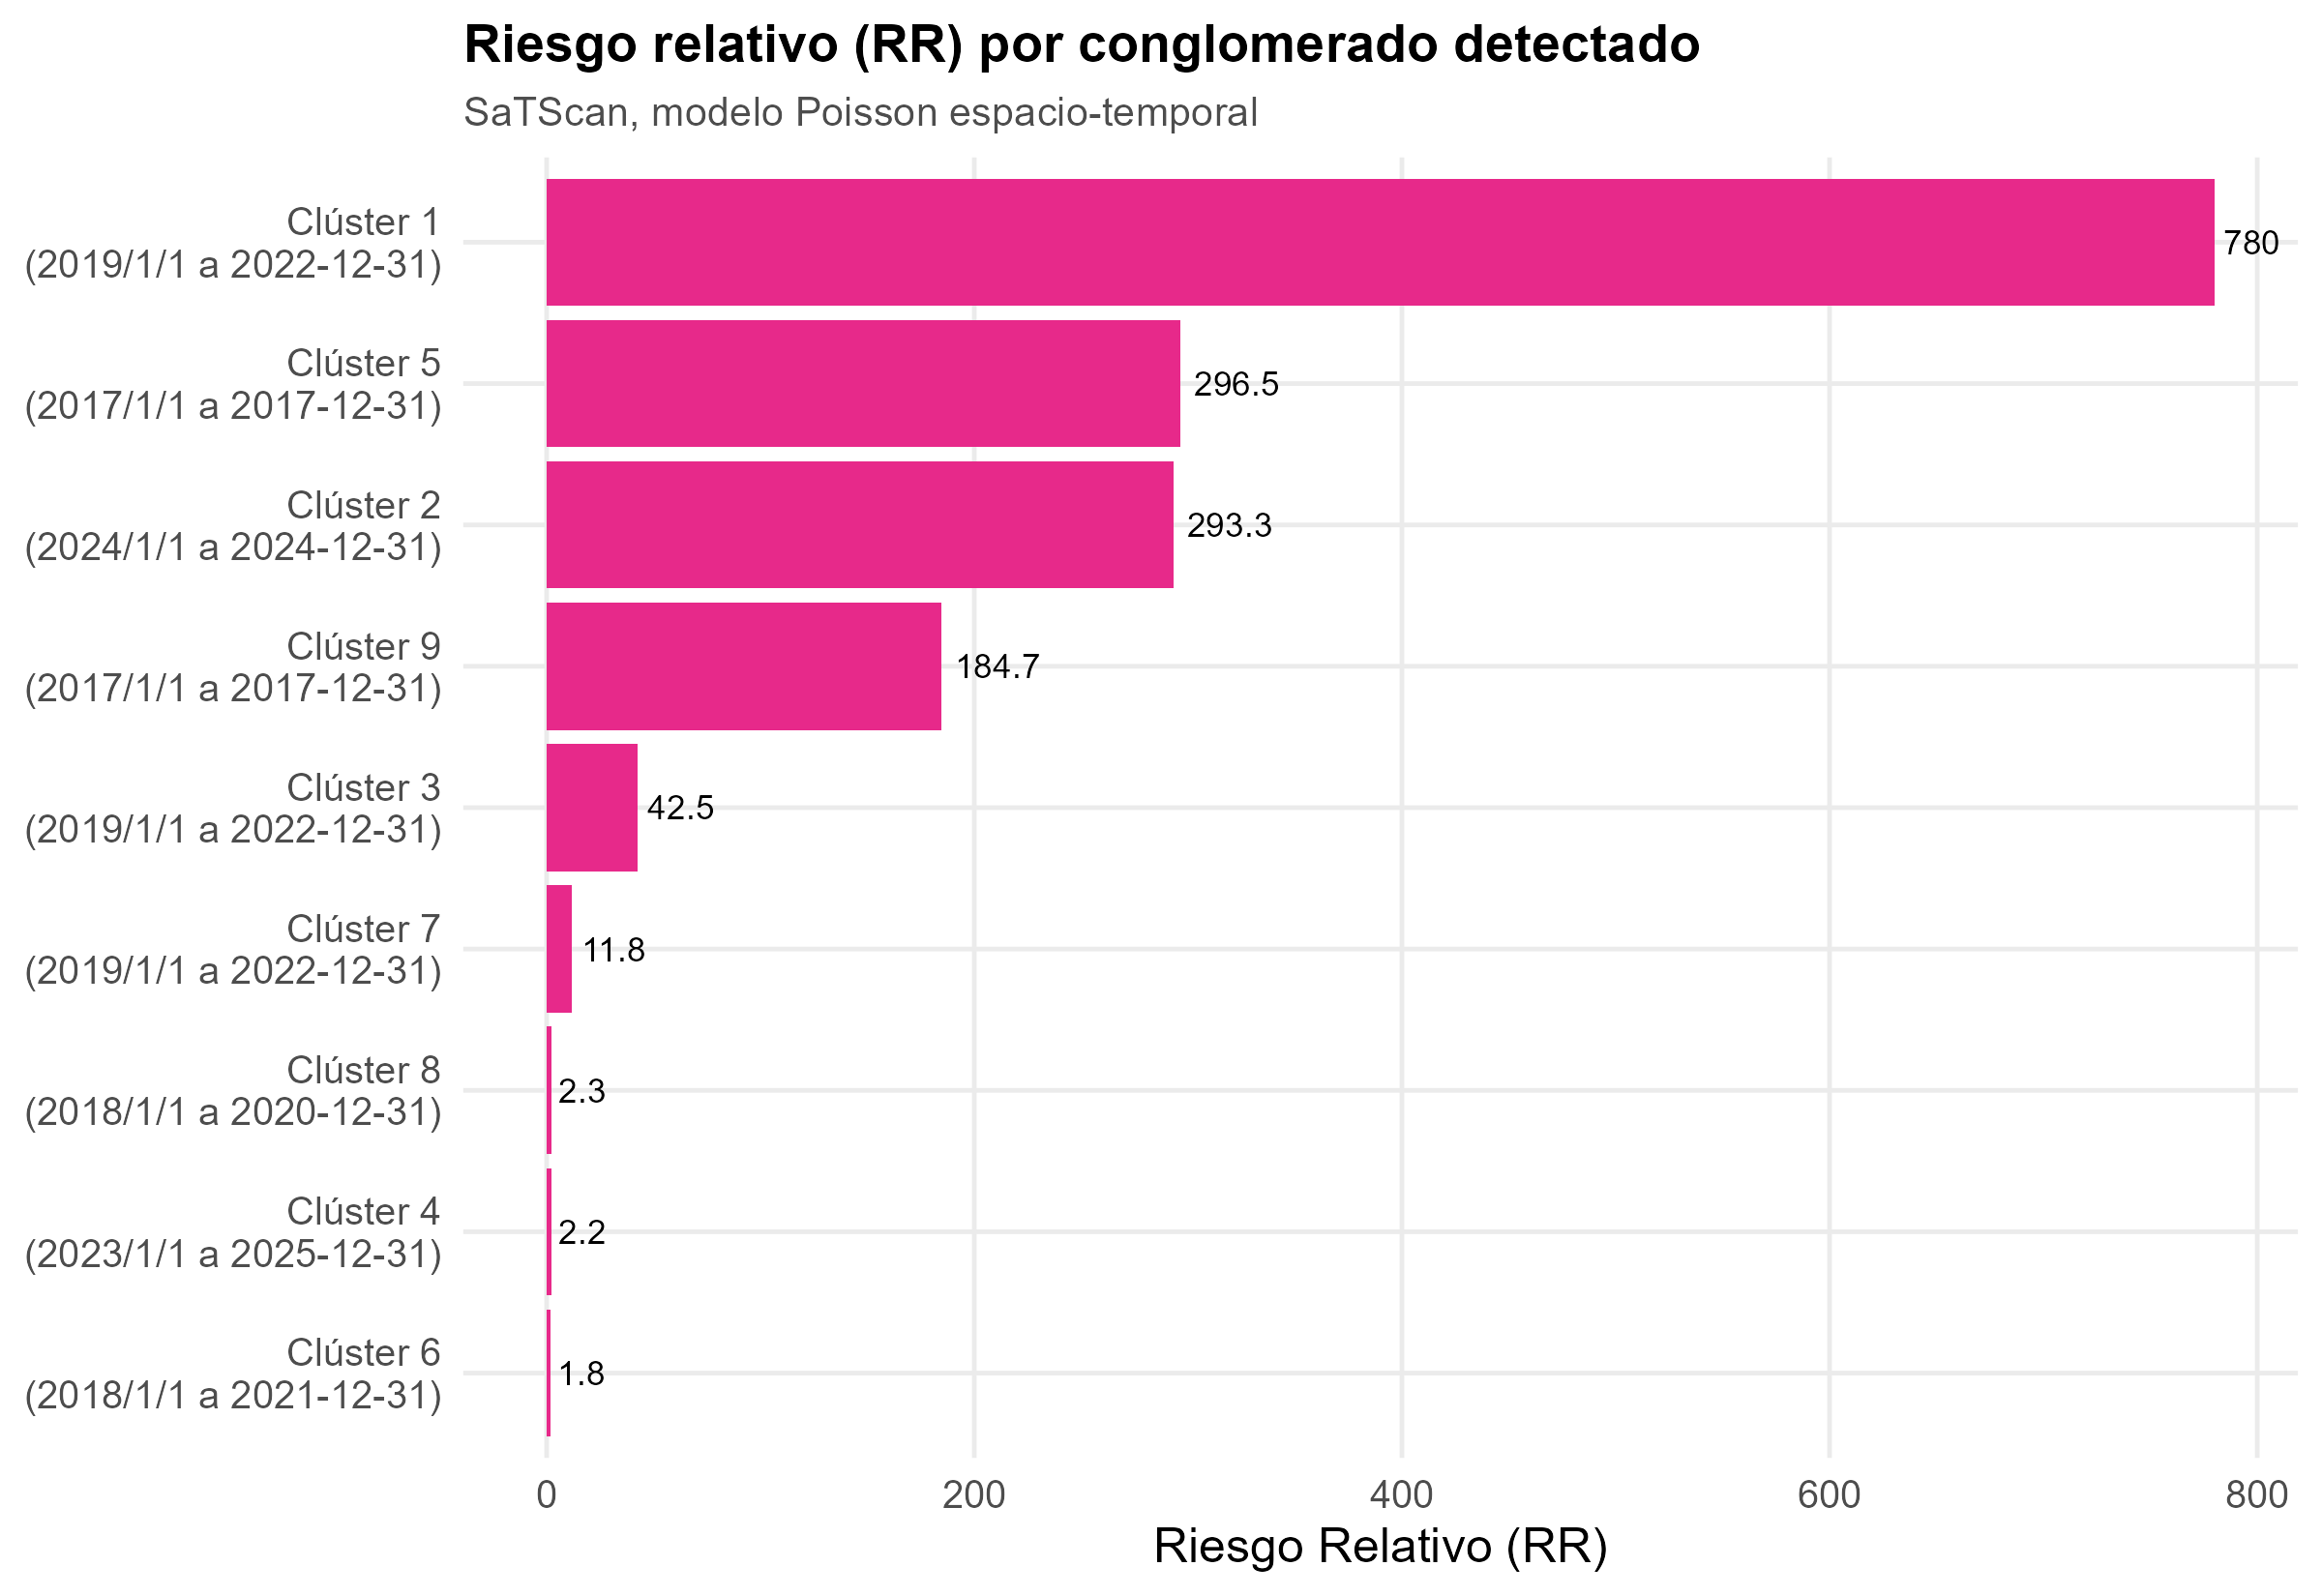
\includegraphics[width=0.85\textwidth]{riesgo_relativo_clusters.png}
		\caption{Relative Risk (RR) and significance (LLR) of the
			9 spatio-temporal clusters.}
		\label{fig:riesgo_relativo}
	\end{figure}
	
	\begin{figure}[htbp]
		\centering
		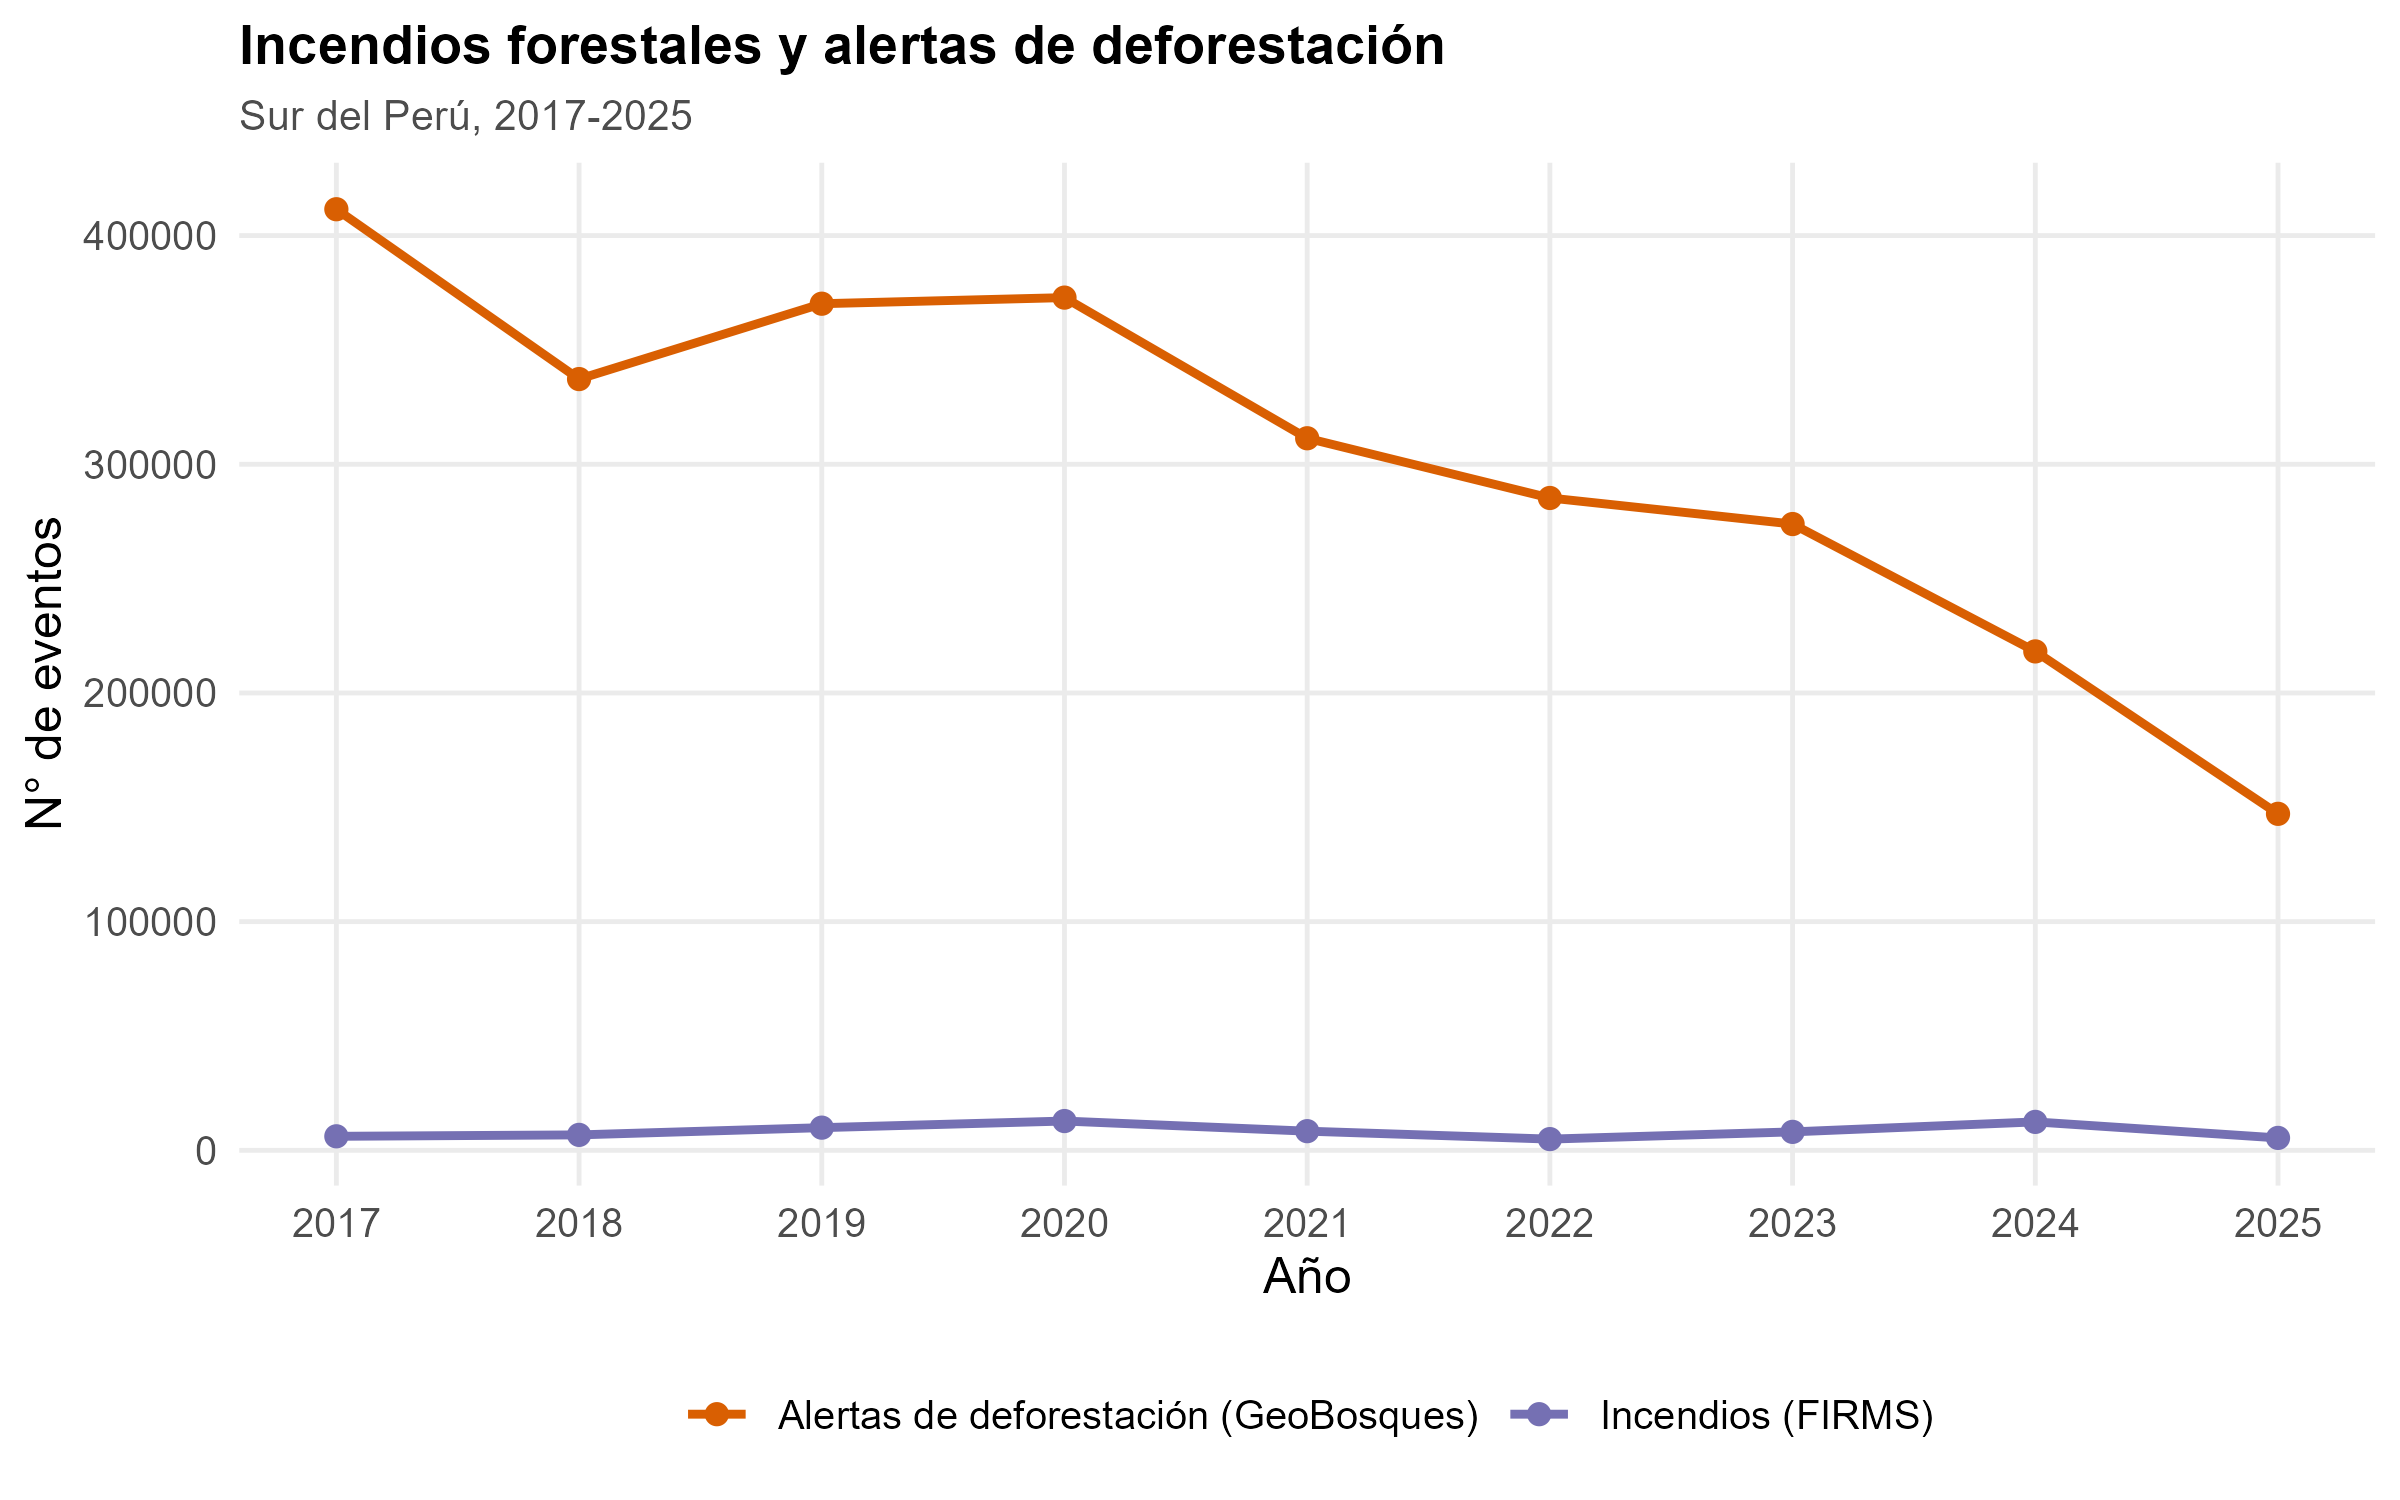
\includegraphics[width=0.85\textwidth]{incendios_vs_deforestacion.png}
		\caption{Bivariate relationship between deforestation alerts and
			forest fires by district.}
		\label{fig:incendios_vs_deforestacion}
	\end{figure}
	
	\subsection{Sensitivity Analysis}
	
	Sensitivity tests restricting the maximum spatial window to
	25\,\% and 30\,\% of the population at risk
	(Figure~\ref{fig:sensibilidad}) demonstrated the stability and
	robustness of the primary cluster ($\text{LLR} > 38{,}000$,
	$\text{RR} \approx 772.3$), ruling out artifacts from spatial
	macro-aggregation. The geometry, temporal period, and relative risk
	of Cluster~1 remained stable across the three window configurations
	evaluated.
	
	\begin{figure}[htbp]
		\centering
		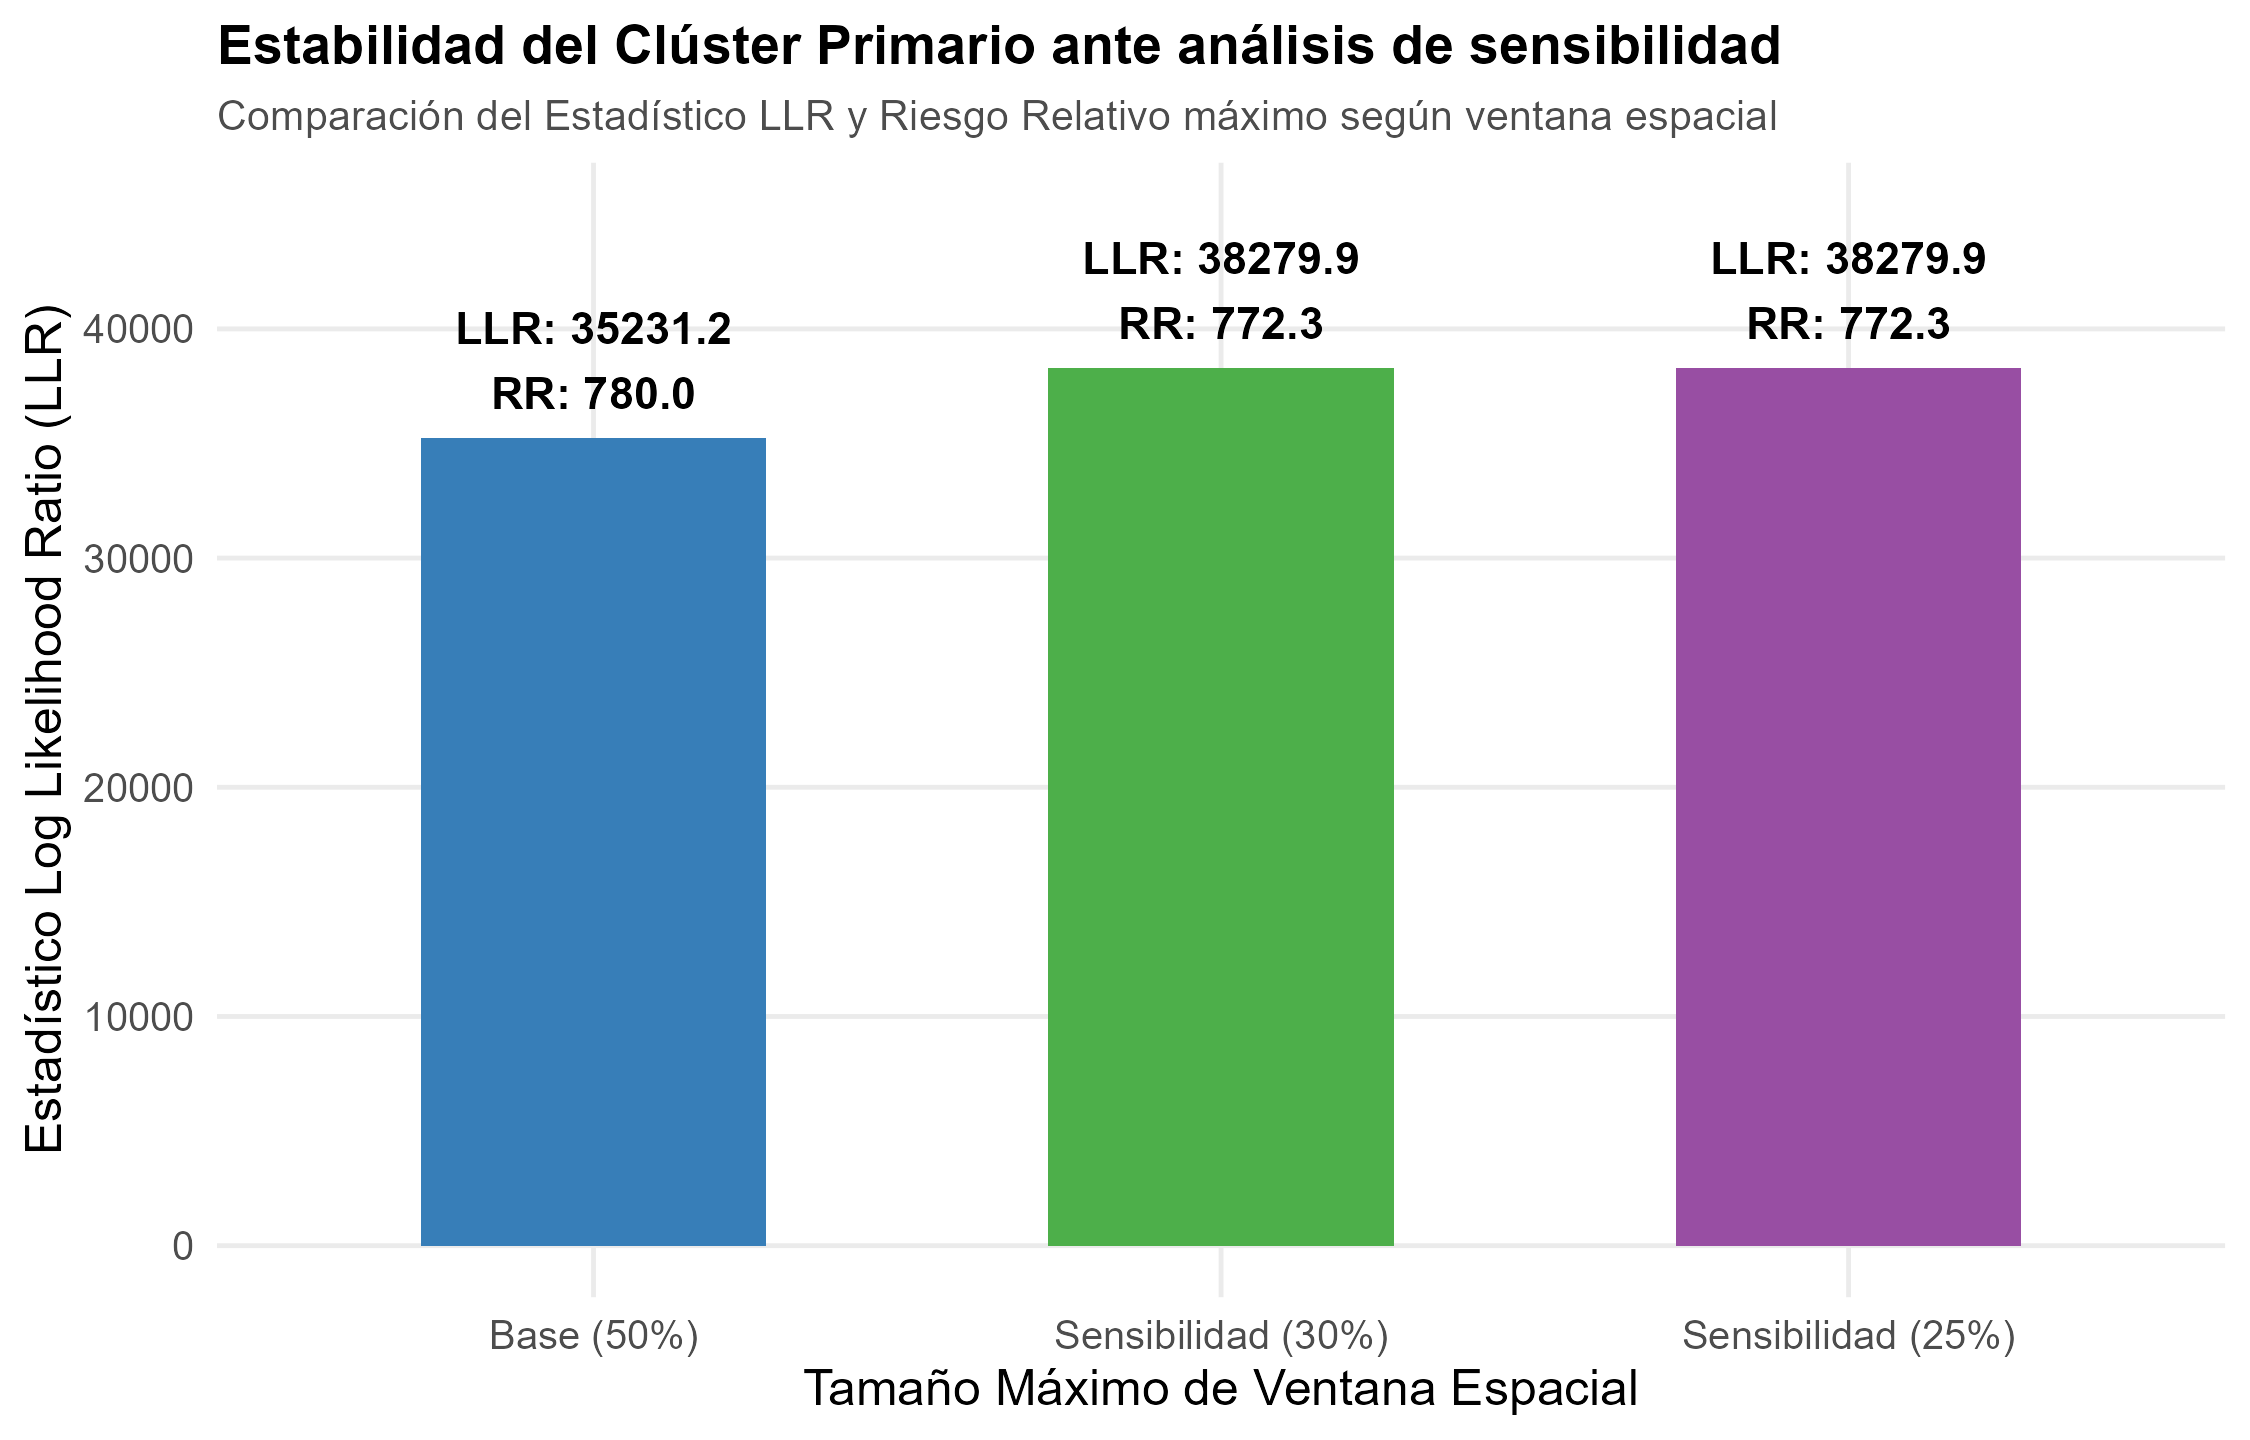
\includegraphics[width=0.82\textwidth]{comparacion_sensibilidad_satscan.png}
		\caption{Stability of the Primary Cluster under sensitivity
			analysis (25\,\%, 30\,\%, and 50\,\% windows).}
		\label{fig:sensibilidad}
	\end{figure}
	
	\section{Discussion}
	
	The findings of this study provide solid empirical evidence of the
	spatio-temporal heterogeneity of forest fires in southern Peru and
	are consistent with patterns documented in other ecogeographic
	contexts of South America. A clear structural duality emerges
	between two differentiated geographic-ecological patterns:
	
	\begin{enumerate}[leftmargin=*, label=\arabic*.]
		\item \textbf{High-Andean Pattern (Cusco--Puno):} Characterized by
		clusters with \textbf{high Relative Risk (RR from 42 to
			780)} but a lower absolute number of hotspots per square
		kilometer. The burning of natural grasslands and
		agricultural stubble at the end of the dry season spreads
		rapidly owing to the strong winds and low relative humidity
		of the puna. M\'ostiga et al.\ (\citeyear{Mostiga2026}) report
		that the Peruvian Andean region accounts for the largest
		share of nationally burned area (2.32\,\%), with a
		significant increasing trend in fire size ($r = 0.49$,
		$p = 0.03$).
		
		\item \textbf{Amazonian Pattern (Madre de Dios):} Characterized by
		clusters with \textbf{high absolute volume (more than
			30{,}000 combined fires across Clusters~4 and 6)} along the
		Interoceanic Highway corridor. Massive deforestation from
		migratory agriculture and mining generates patches of
		felled biomass that are burned during August and September.
		This pattern is analogous to that documented by Valente
		\& Laurini\ (\citeyear{Valente2023}) in the Brazilian Amazon,
		where road proximity is the main spatial driver of fire
		occurrence.
	\end{enumerate}
	
	The strong bivariate autocorrelation ($I = 0.6019$) confirms that
	land-use change (deforestation) acts as the main spatial catalyst
	of fire, in line with findings by Ma et al.\ (\citeyear{Ma2022}) for the
	Amazon, where pasture area and forest-fragmentation edge density
	are the strongest predictors of fire intensity. Raiol et
	al.\ (\citeyear{Raiol2026}) confirm that pasture expansion significantly
	increases hotspot rates ($p = 0.04$, Sen's slope $= +15.31$
	hotspots/year). This suggests that fire-prevention policies by
	SERFOR and MINAM should integrate environmental enforcement against
	deforestation as a direct measure for reducing forest-fire risk.
	
	\subsection*{Study Limitations}
	
	This study presents a set of methodological and data limitations
	that should be considered when interpreting the results:
	\begin{enumerate}[leftmargin=*, label=(\roman*)]
		\item MODIS hotspots have a spatial resolution of 1~km, which may
		result in under-detection of small-extent fires in areas
		with persistent cloud cover (December--March).
		\item The VIIRS and MODIS sensors generate independent records for
		the same thermal event, so there remains a residual risk of
		hotspot duplication despite the filtering applied.
		\item The analysis is restricted to 237 districts in southern
		Peru, limiting generalization at the national level.
		\item The bivariate Moran's Index measures static spatial
		association and does not imply causality; spatio-temporal
		panel models are required to establish formal causal
		relationships.
		\item The exploratory sensitivity analysis was run with 99 Monte
		Carlo replications, sufficient for the geometric exploration
		of clusters but not for reporting definitive $p$-values for
		publication.
	\end{enumerate}
	
	\section{Conclusions}
	
	\begin{enumerate}[leftmargin=*, label=\arabic*.]
		\item \textbf{Nine statistically significant spatio-temporal
			clusters of forest fires} were detected in southern Peru
		between 2017 and 2025.
		
		\item Fire occurrence exhibits critical seasonality concentrated
		in the \textbf{July--October period (89.51\,\%)}, peaking in
		\textbf{September (39.01\,\%)}, with interannual peaks in
		\textbf{2020 and 2024}.
		
		\item Bivariate spatial autocorrelation analysis ($I = 0.6019$,
		$p = 0.001$) demonstrates a direct spatial association
		between deforestation alerts and hotspot occurrence in
		neighboring districts.
		
		\item Sensitivity tests (25\,\% and 30\,\%) confirm the robustness
		of the Cusco--Puno Primary Cluster and of the Amazonian
		clusters in Madre de Dios under different spatial-window
		assumptions.
		
		\item These results allow spatial prioritization of Madre de Dios
		(high absolute event mass) and the Cusco--Puno interface
		(high relative risk) for the timely deployment of response
		resources and environmental monitoring by SERFOR and MINAM.
	\end{enumerate}
	
	\section*{Acknowledgements}
	
	The author thanks NASA's Fire Information for Resource Management
	System (FIRMS) for open access to VIIRS/MODIS hotspot data, and
	Peru's Ministry of the Environment (MINAM) for the public
	availability of the GeoBosques forest-cover monitoring platform.
	The author also thanks the National Forest and Wildlife Service
	(SERFOR) for the national technical reports on forest fires.
	Statistical analysis was carried out using free and open-source
	software: R~v4.4.x and SaTScan~v10.3.3.
	
	\bibliographystyle{elsarticle-harv}
	\bibliography{referencias}
	
	\section*{Declaration of Competing Interest}
	The author declares that he has no known competing financial interests or personal relationships that could have appeared to influence the work reported in this paper.
	
	\section*{Funding}
	This research did not receive any specific grant from funding agencies in the public, commercial, or not-for-profit sectors.
	
	\section*{Data Availability}
	Hotspot data are available through NASA's FIRMS system (\url{https://firms.modaps.eosdis.nasa.gov/}). Deforestation alerts originate from GeoBosques-MINAM (\url{https://geobosques.minam.gob.pe/}). District boundaries are available through INEI. The SaTScan parameter files (\texttt{.prm}), R processing scripts, and spatial result files (\texttt{.shp}) generated in this study are available from the corresponding author upon reasonable request.
	
\end{document}
